\documentclass[11pt,letterpaper]{article}
\input{headings}
\usepackage{soul}

\newcommand \recipeName {Zucchini Chorizo Soup}
\newcommand \fileName {ZucchiniChorizoSoup}

\chead{\recipeName}

\begin{document}
\input{title}

Sometimes a recipe just happens because of the things that happen to be around the house. This is one such recipe. It turned out really good. There are some principles that are used here that can be used in several other recipes with similar ingredients. Zucchini are green Summer squashes. In the heat of the Summer they can grow very rapidly and it is all too easy to overlook one when harvesting and you end up with a very large overgrown zucchini with a tough green peel and mushy seed inside. Unless it is cooked carefully, such a squash is not pleasant to eat. I have developed a recipe to quickly sautee zucchini in a flavourful oil base --- it is similar to the stir frying in Chinese cooking, but I do not use the combination of strong flavours from soy sauce, fish sauce, or bean paste. For this recipe I had some spicy Spanish chorizo in the fridge and  I was harvesting the remaining of my carrots from the garden. Using cooked rice to make a creamy soup is a technique that I have seen in Thai soups.

\begin{description}

\item[Ingredients:]\ \\
	\begin{itemize}
	\item 1/2 of an overgrown zucchini (or two regular zucchinis)
	\item 4 or 5 fresh (not smoked) Spanish chorizo sausages
	\item 5 cloves of garlic
	\item 500 grams of carrots
	\item 1 tablespoon of canola oil
	\item hot water
	\item salt to taste 
	\item  two tablespoons of chopped parsley
	\end{itemize}

\item[Procedure:]\ \\
	\begin{enumerate}
	\item {\bf Prepare the Zucchini and the Carrots}
	\begin{itemize}
	\item Cut the zucchini in half and use a spoon to remove and discard the seeds and the soft pulp around the seeds.
	\item Peel the tough green skin of the overgrown zucchini (there is no need to peel if using normal zucchini with tender skin.
	\item Cut the zucchini into a small dice (about 1 cm cube pieces).
	\item Lightly sprinkle the diced zucchini with salt and put in a bowl.
	\item Peel and dice the carrots and put in a separate bowl.
	\item Lightly sprinkle the carrots with salt.
	\item Both the zucchini and the carrots should stay in the salt for at least 20 minutes.
	\end{itemize}
	\item {\bf Preparing the sausage}
	\begin{itemize}
	\item Remove the sausage from the casings.
	\item Cut each sausage in half and then cut each half into small pieces.
	\item Using a heavy bottom pan over moderate heat, heat up the oil until it is shimmering. 
	\item Quickly sautee the sausage until it changes colour, but do not attempt to obtain a darker brown colour because it would result in dry and tough pieces of sausage.
	\item Remove the sausage from the pan and put on a stainer over a bowl to collect that fat.
	\end{itemize}
	\item{\bf Sautee the zucchini}
	\begin{itemize}
	\item The salt has extracted some water from the zucchini. Put the zucchini on a strainer and discard the water.
	\item Peel the garlic cloves and cut in half.
	\item Transfer the fat that was drained from the sausages back into the pan. 
	\item Warm the fat over moderate heat until shimmering.
	\item Add the halved garlic cloves and stir fry for 20 to 30 seconds until you can smell their fragrance
	\item Immediately add all the drained zucchini to the hot pan and stir fry for about a minute.
	\item Remove the zucchini and garlic to a strainer over a bowl to collect the fat.
	\item The zucchini will appear to not be cooked at this point. 	
	\end{itemize}
	\item{\bf Preparing the soup base}
	\begin{itemize}
	\item Put a strainer over a bowl and put the diced carrots in the strainer to drain the water -- reserve the water from the carrots.
	\item Transfer the fat drained from the zucchini back to the pan.
	\item Put the drained diced carrots in the hot pan and stir fry for several minutes until you notice light browning in the carrots.
	\item Add the reserved carrot water and add one cup of hot water.
	\item Simmer the carrots for about ten minutes until they are tender enough to be processed.
	\item Meanwhile carefully remove each of the garlic pieces from the cooked diced zucchini and transfer the garlic pieces to a blender.
	\item Once the carrots are tender, transfer the entire content of the pan to the blender.
	\item Transfer about 1/3 of cooked dice zucchini to the blender.
	\item Add the one cup of cooked rice to the blender.
	\item Blend until completely smooth. You may need to add small amounts of hot water to the mixture to obtain a smooth soup base.
	\end{itemize}
	\item{\bf Finishing the soup}
	\begin{itemize}
	\item Transfer the soup base back to the pan and set over moderate heat.
	\item Add more hot water if needed to obtain a creamy consistency.
	\item Add the sausage to the pot.
	\item After the sausage is warmed up, transfer the diced zucchini to the pot and just warm it through.
	\item Add the chopped parsley and serve with some warmed up crusty bread.
	\end{itemize}
	\end{enumerate}
\end{description}
\begin{table}
\begin{tabular}{cccc}
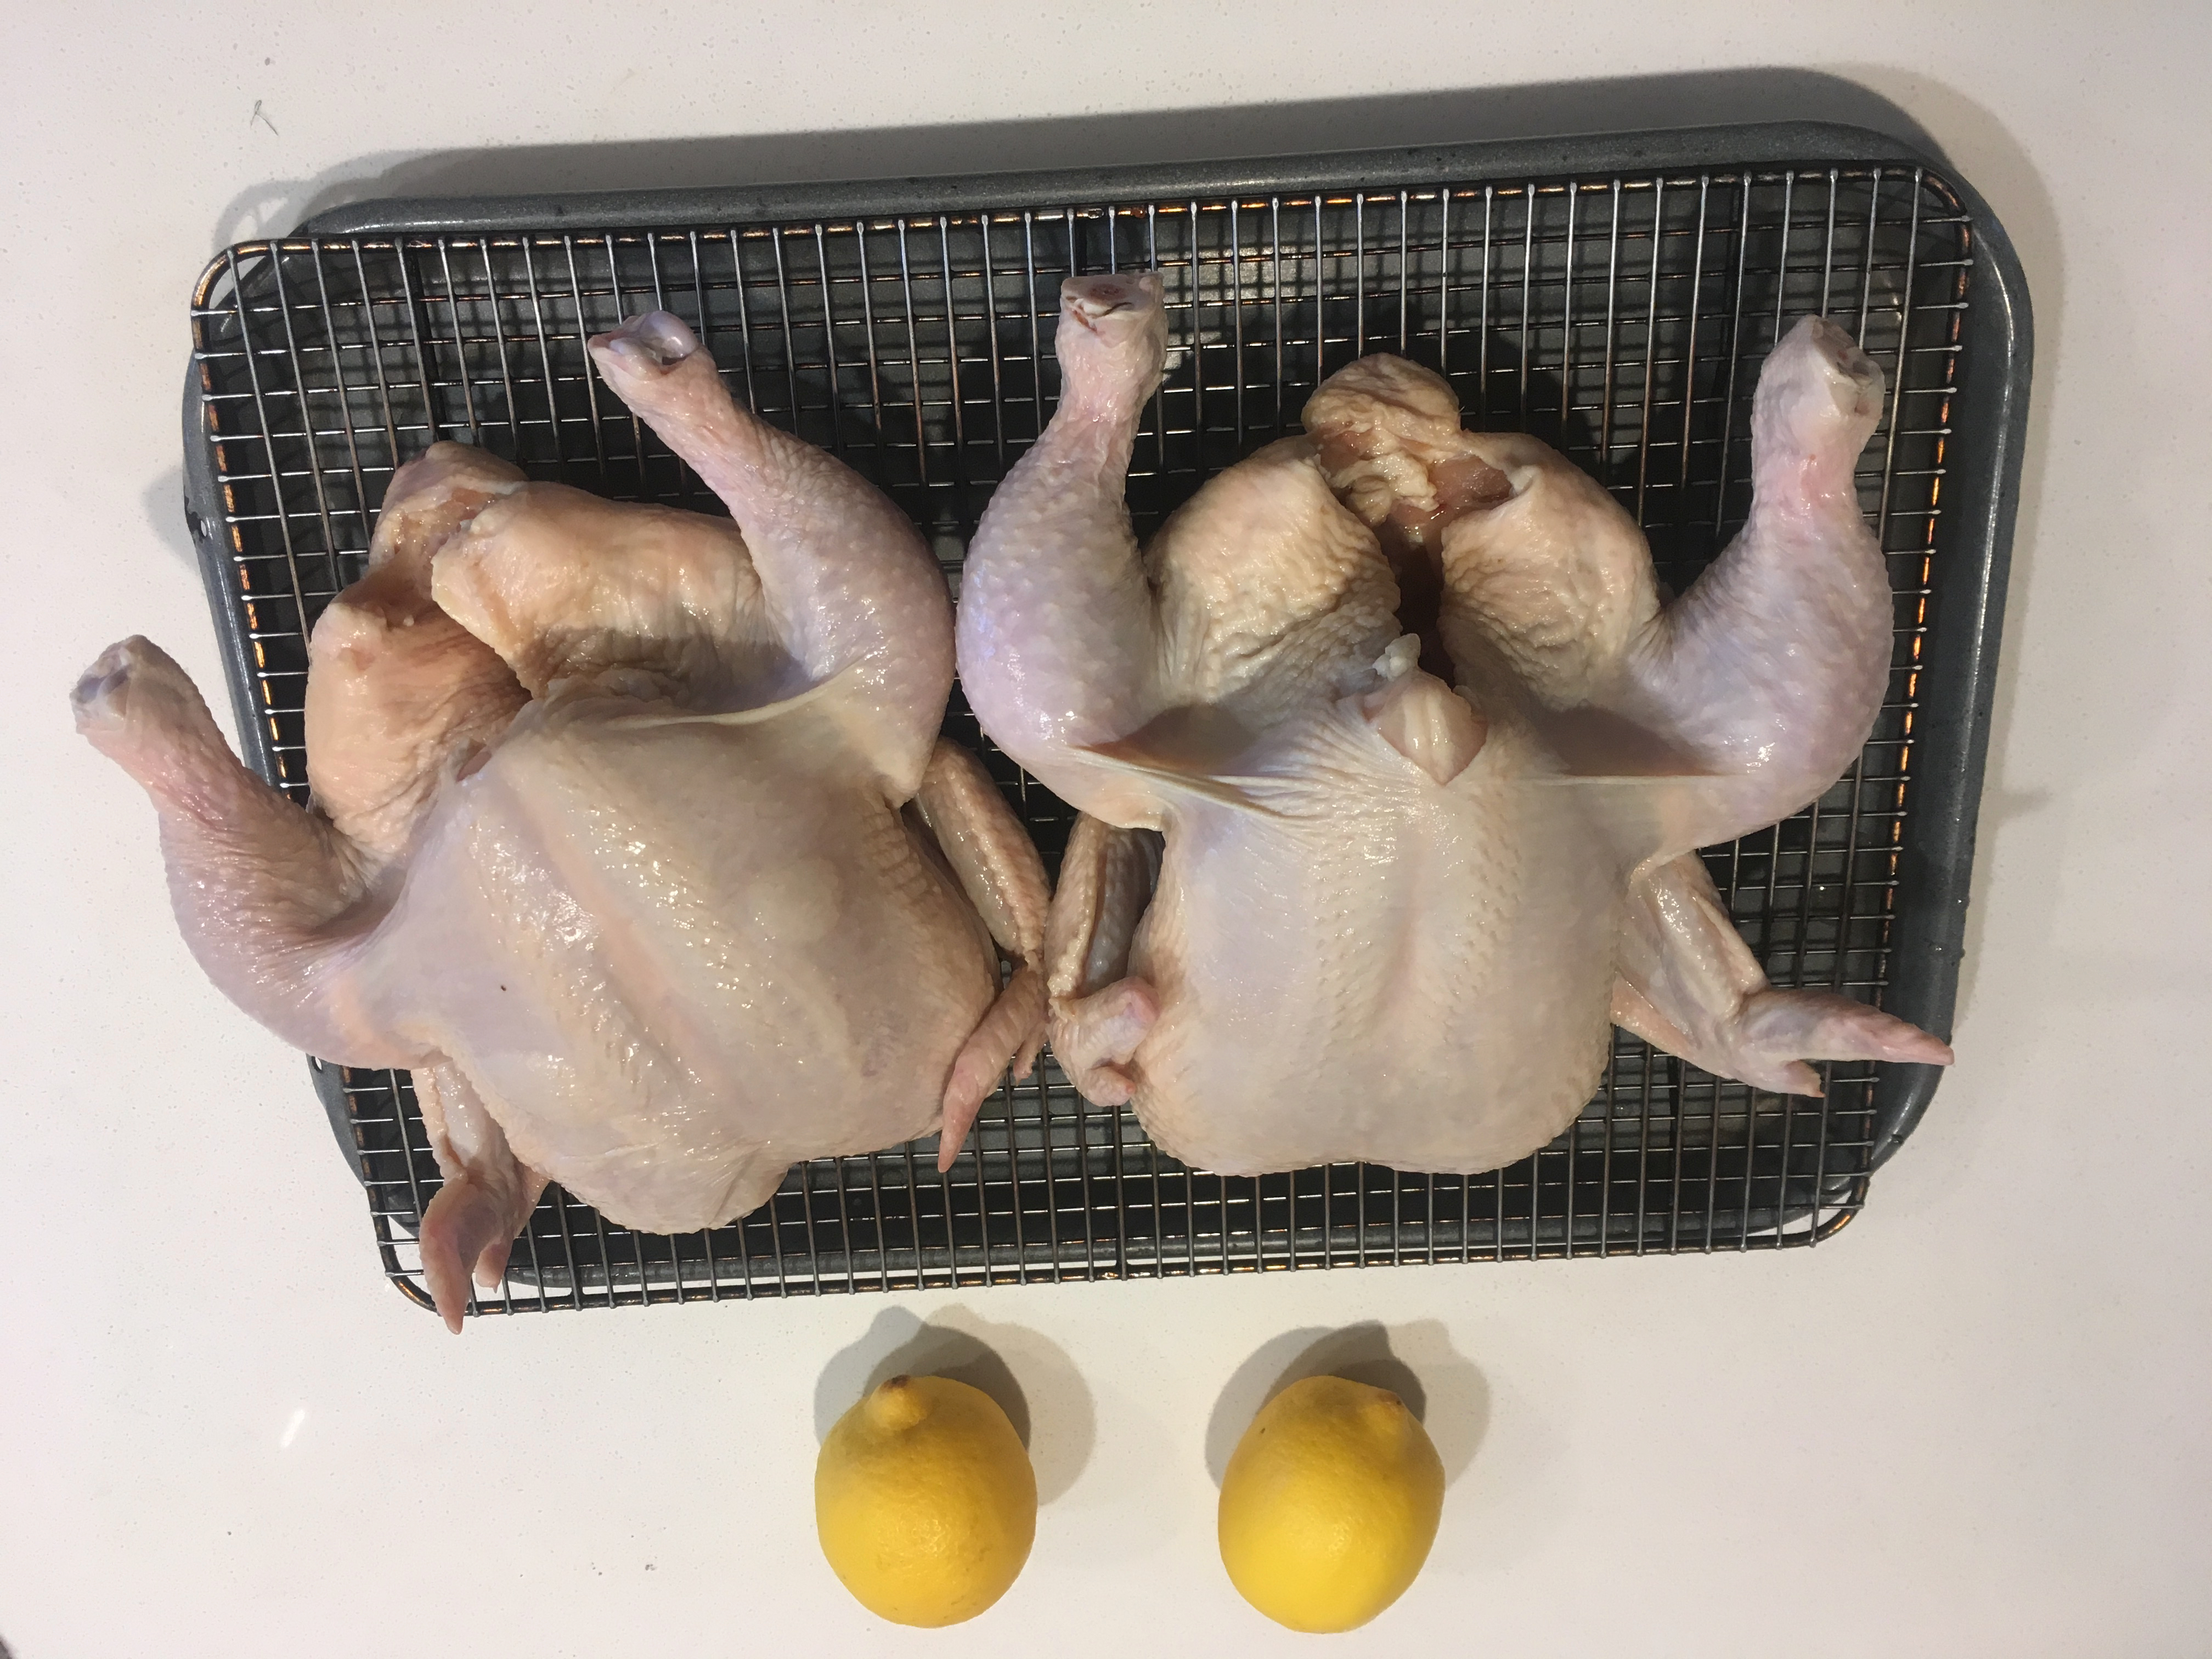
\includegraphics[width=0.25\textwidth]{\imageDir/\fileName/IMG_3197.jpg} &
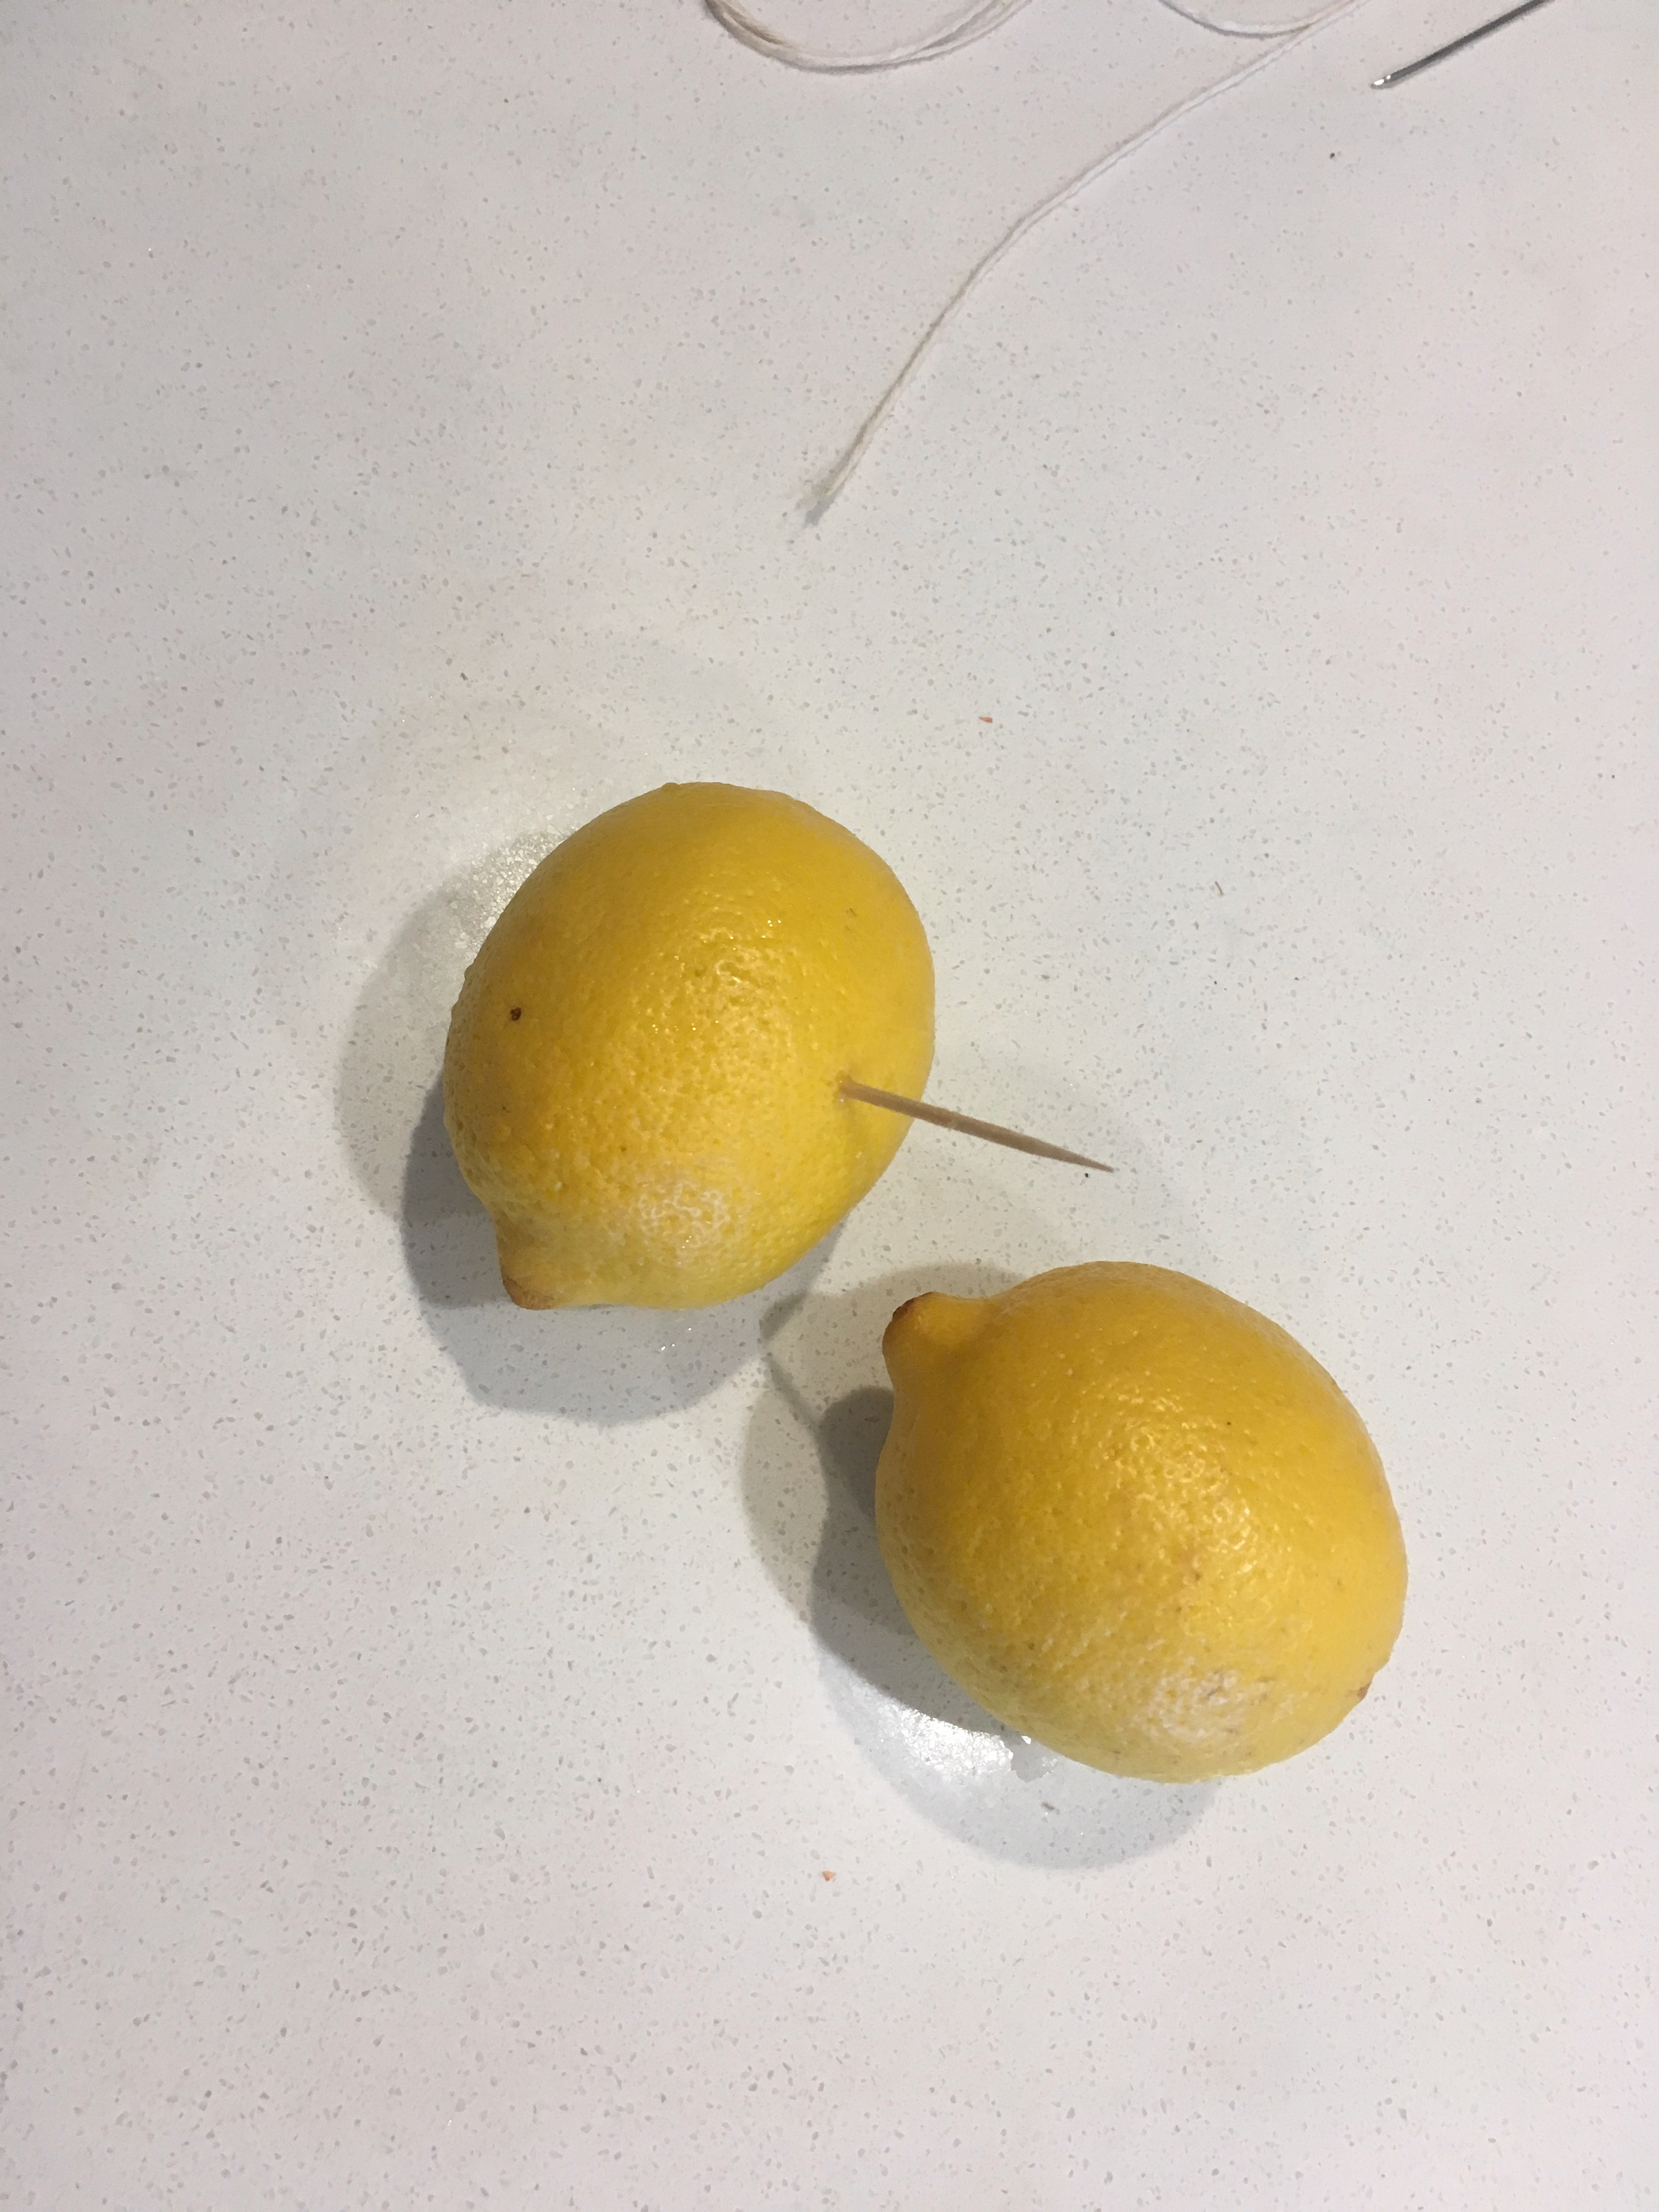
\includegraphics[width=0.25\textwidth]{\imageDir/\fileName/IMG_3212.jpg} &
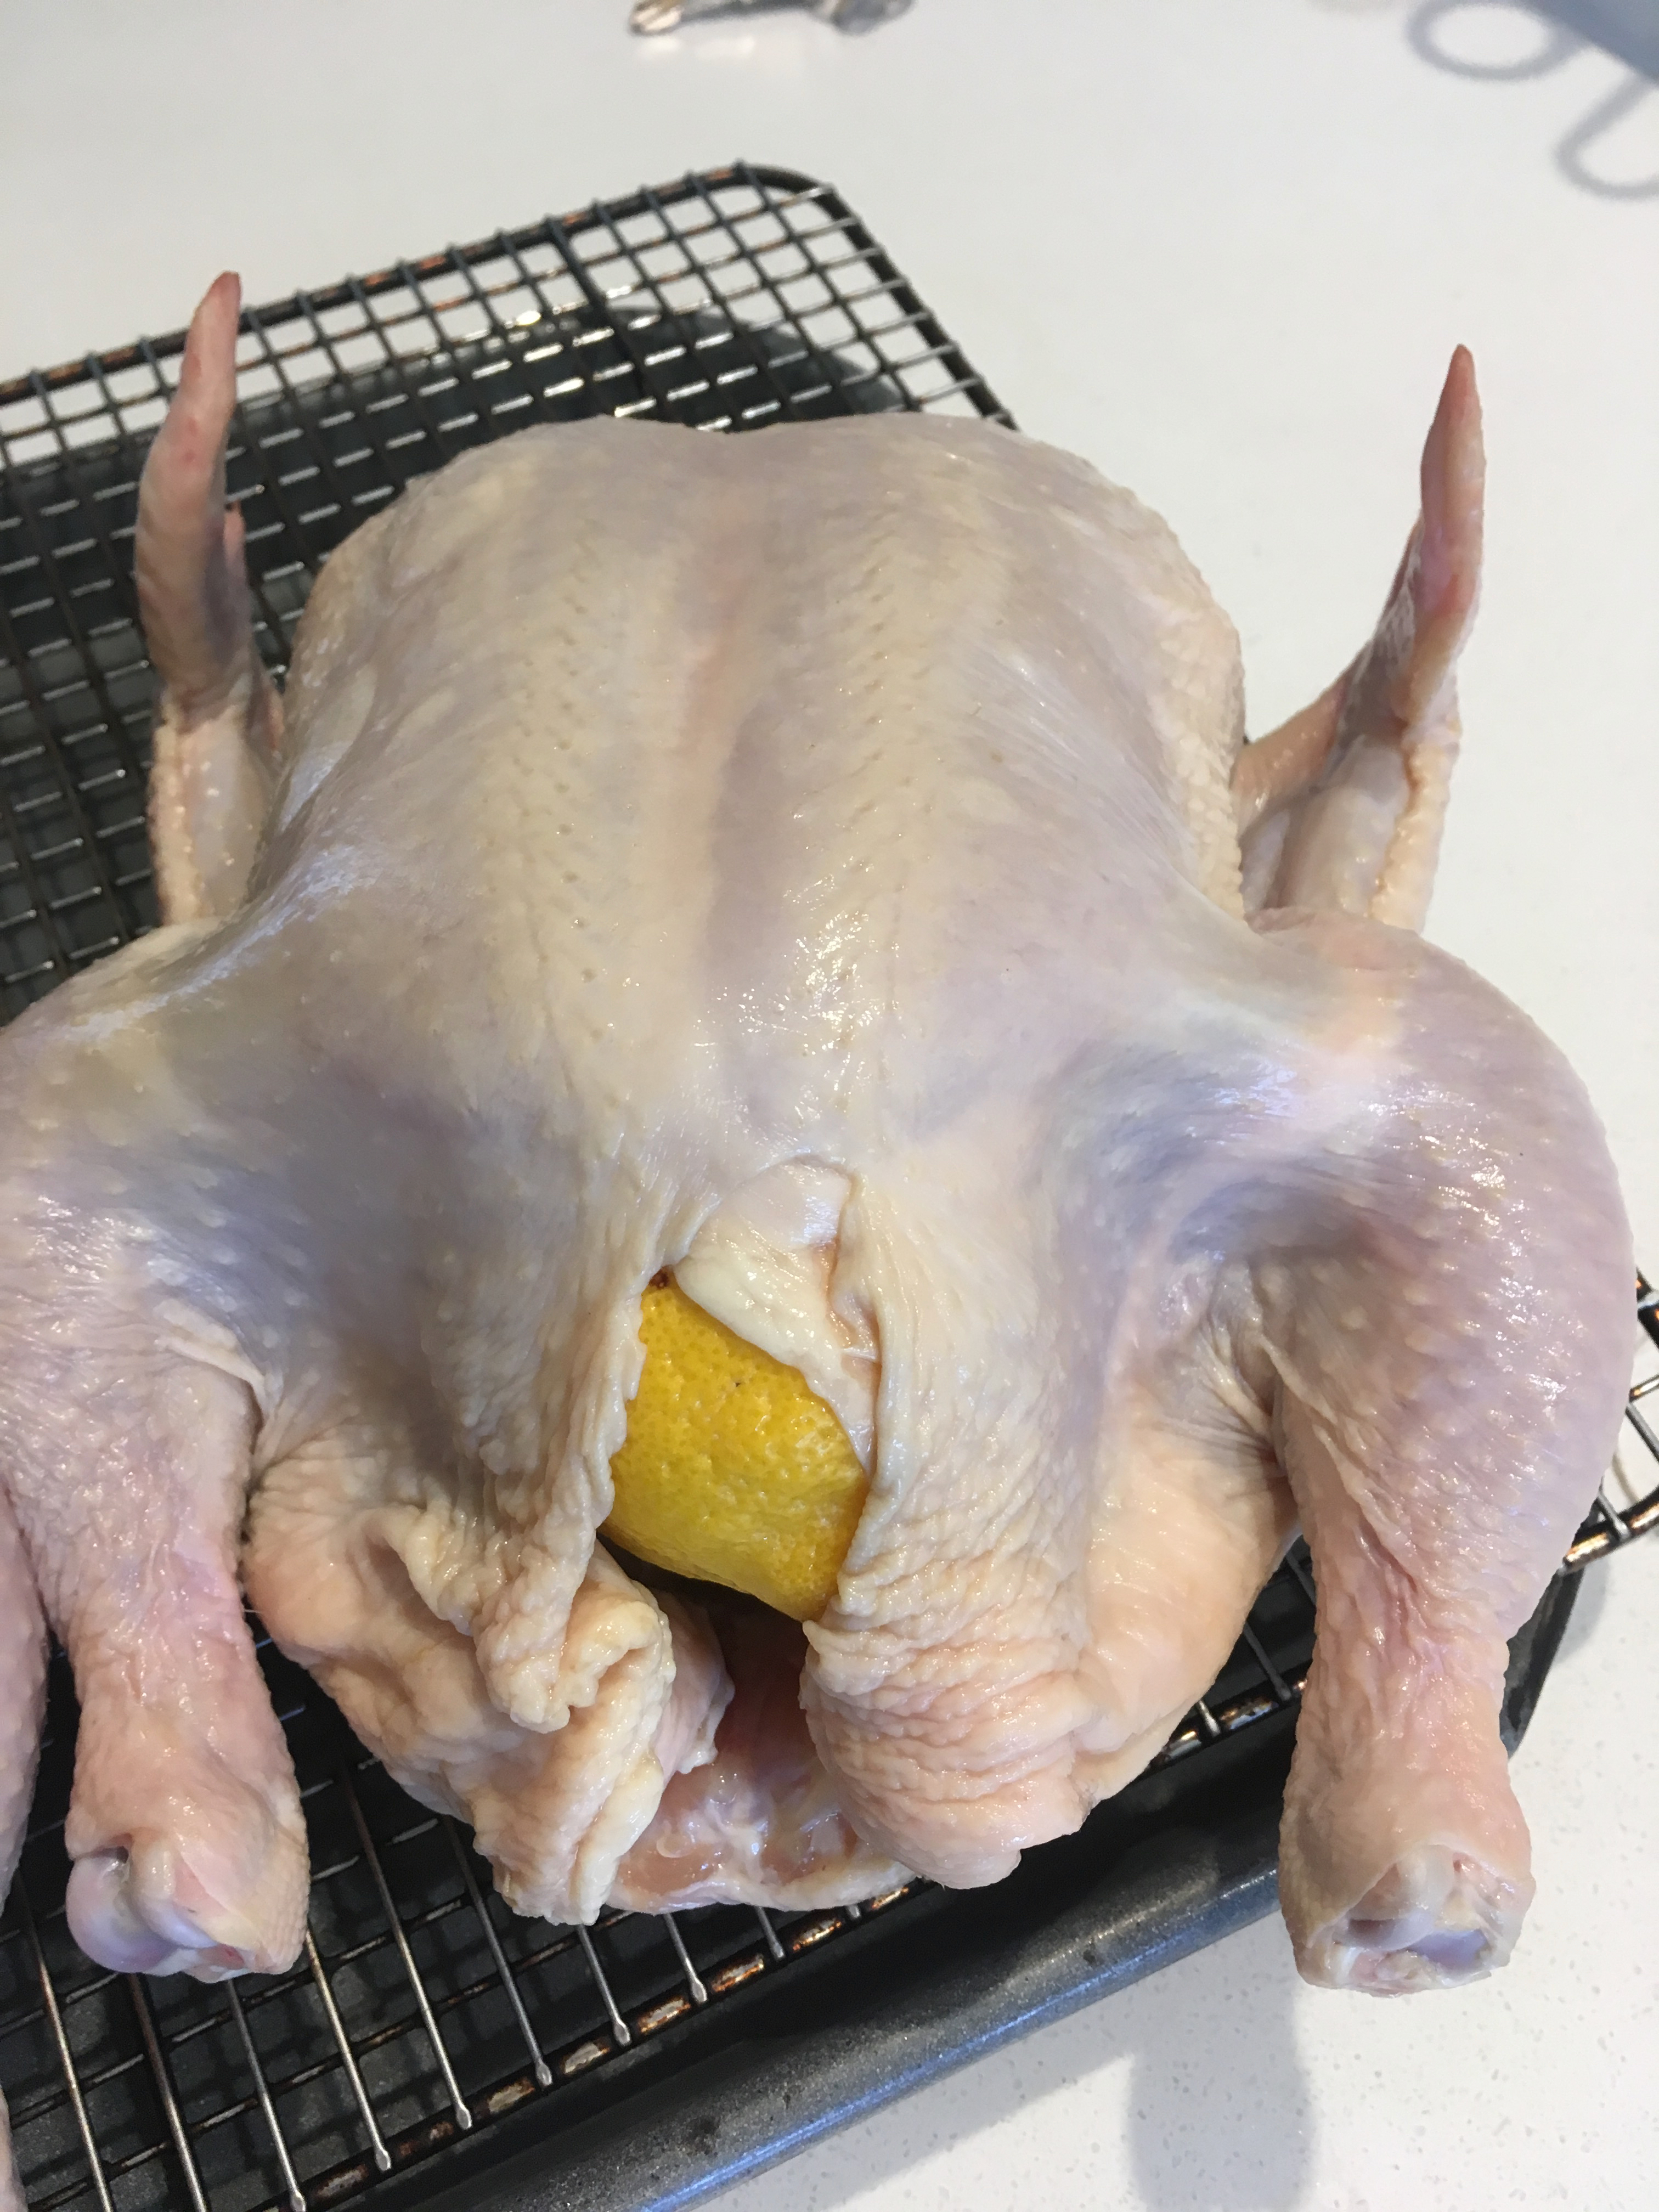
\includegraphics[width=0.25\textwidth]{\imageDir/\fileName/IMG_3213.jpg} \\
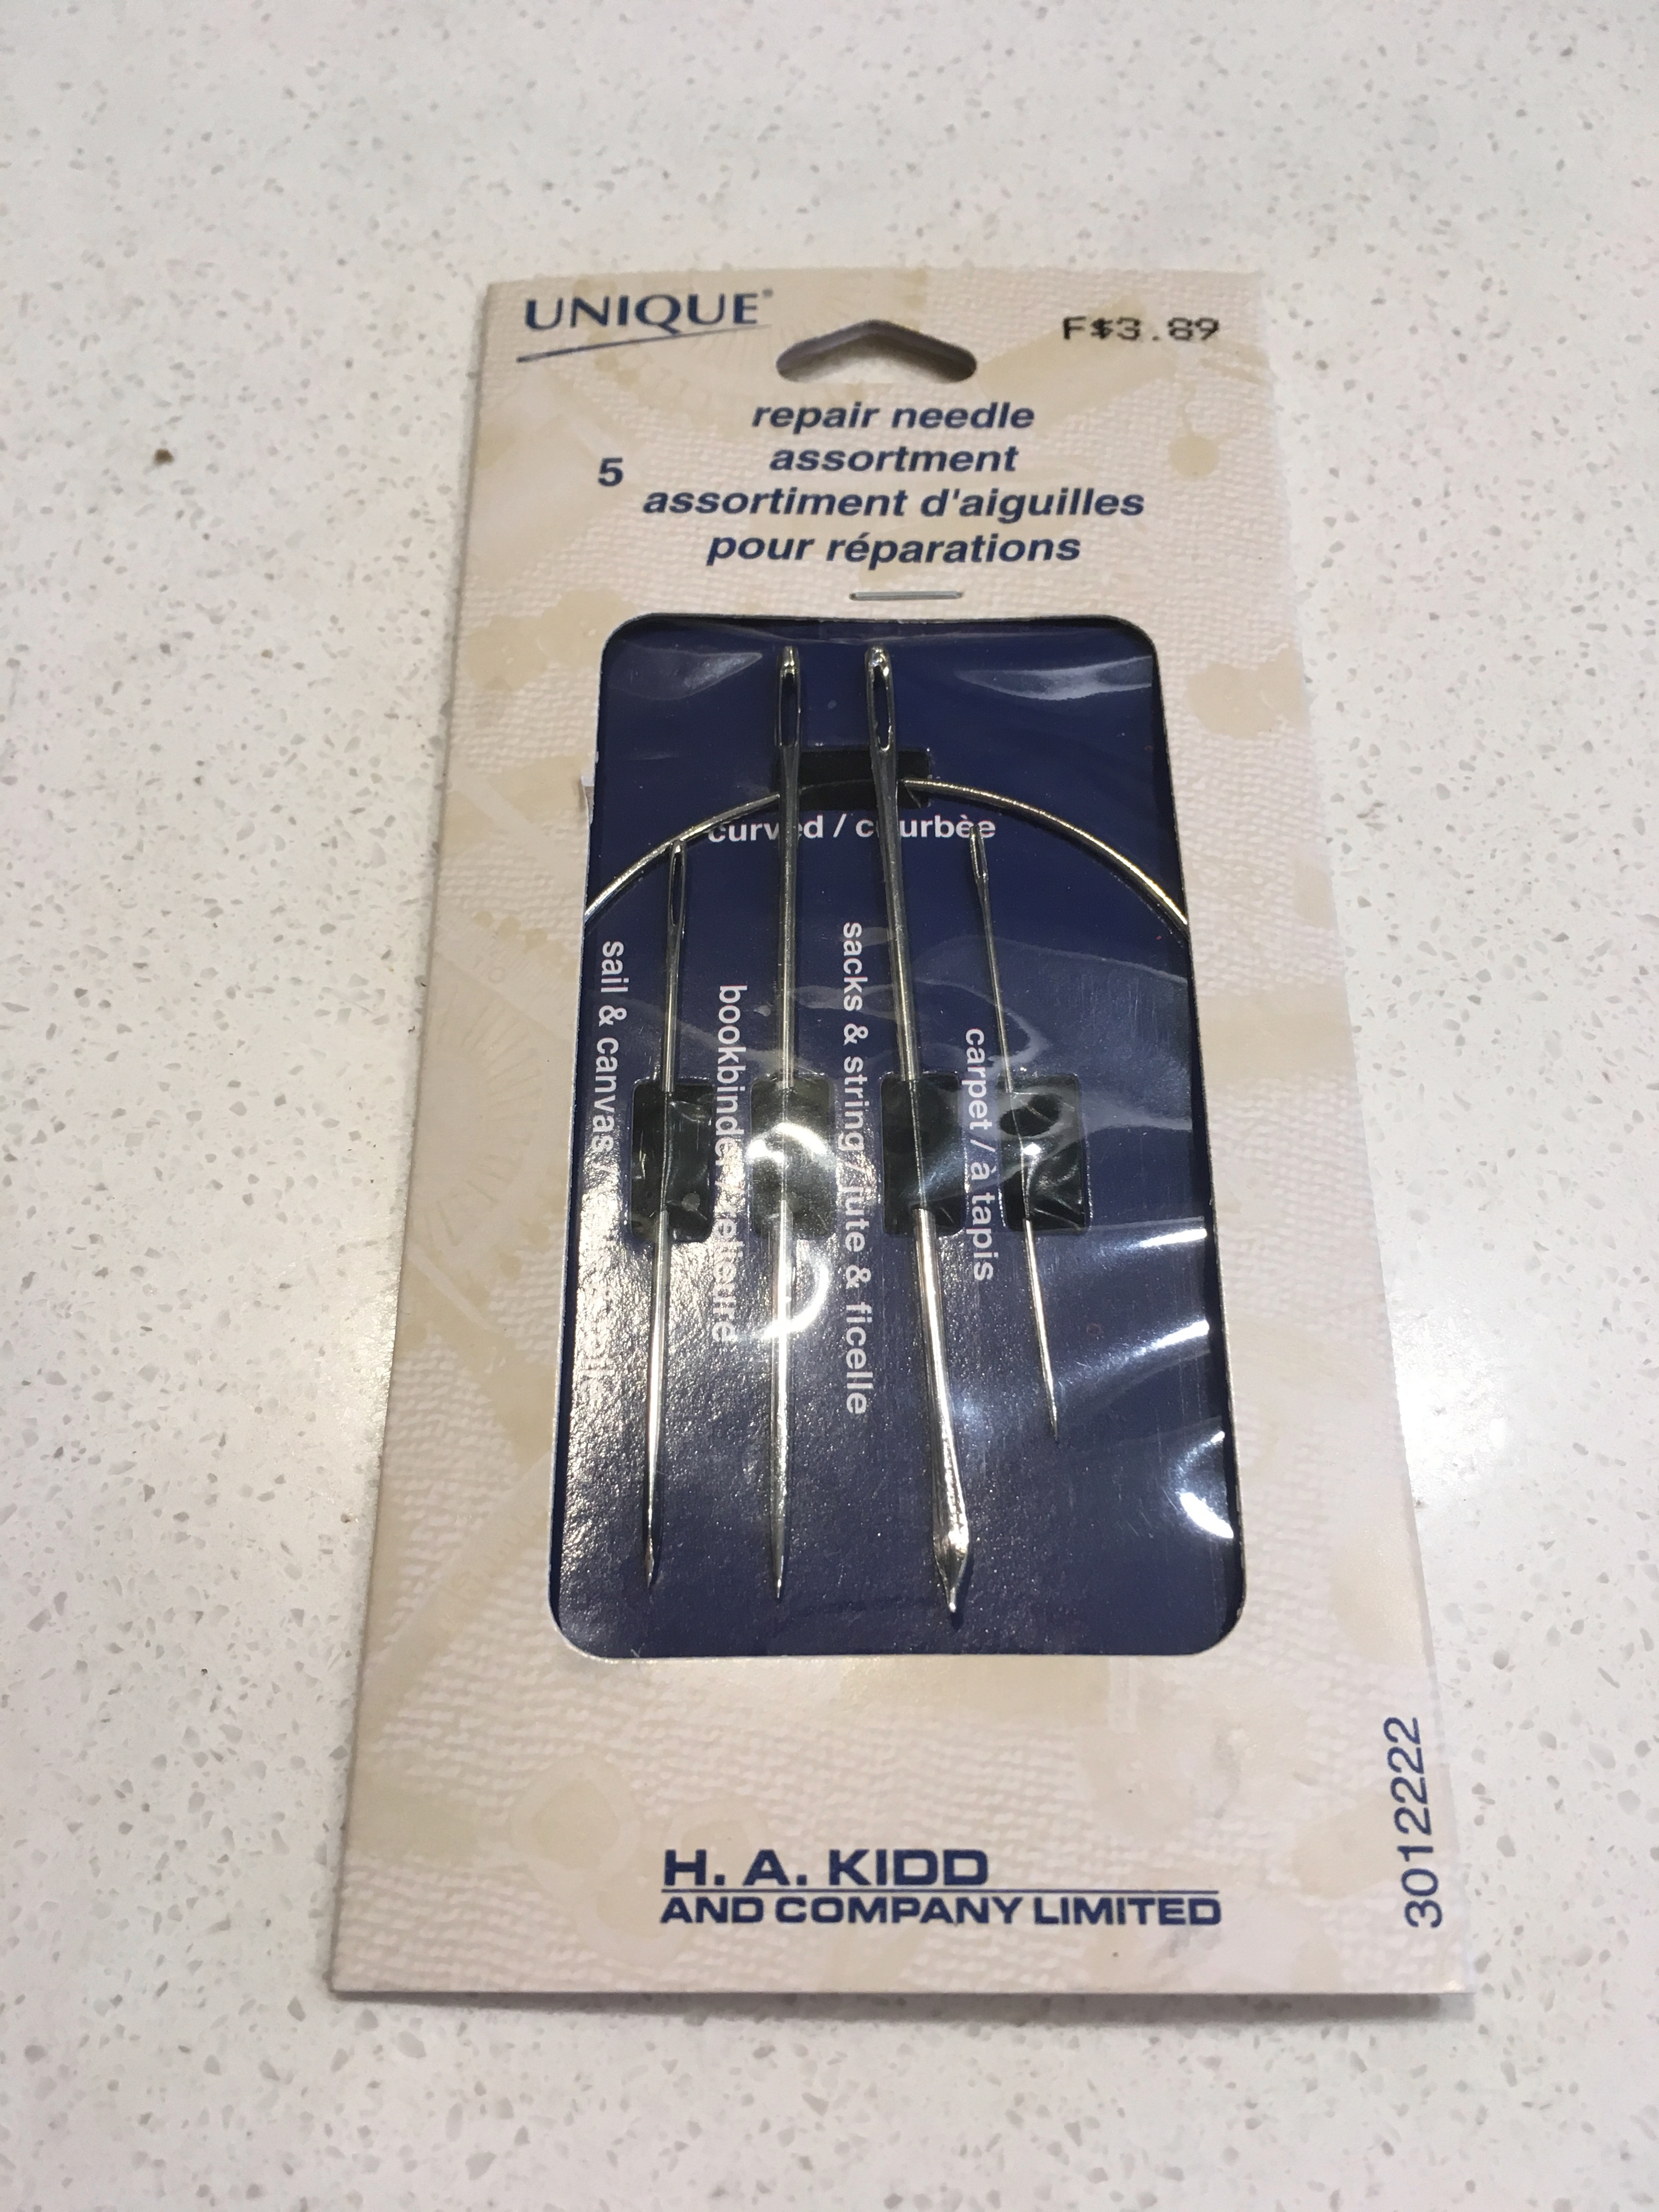
\includegraphics[width=0.25\textwidth]{\imageDir/\fileName/IMG_3206.jpg} &
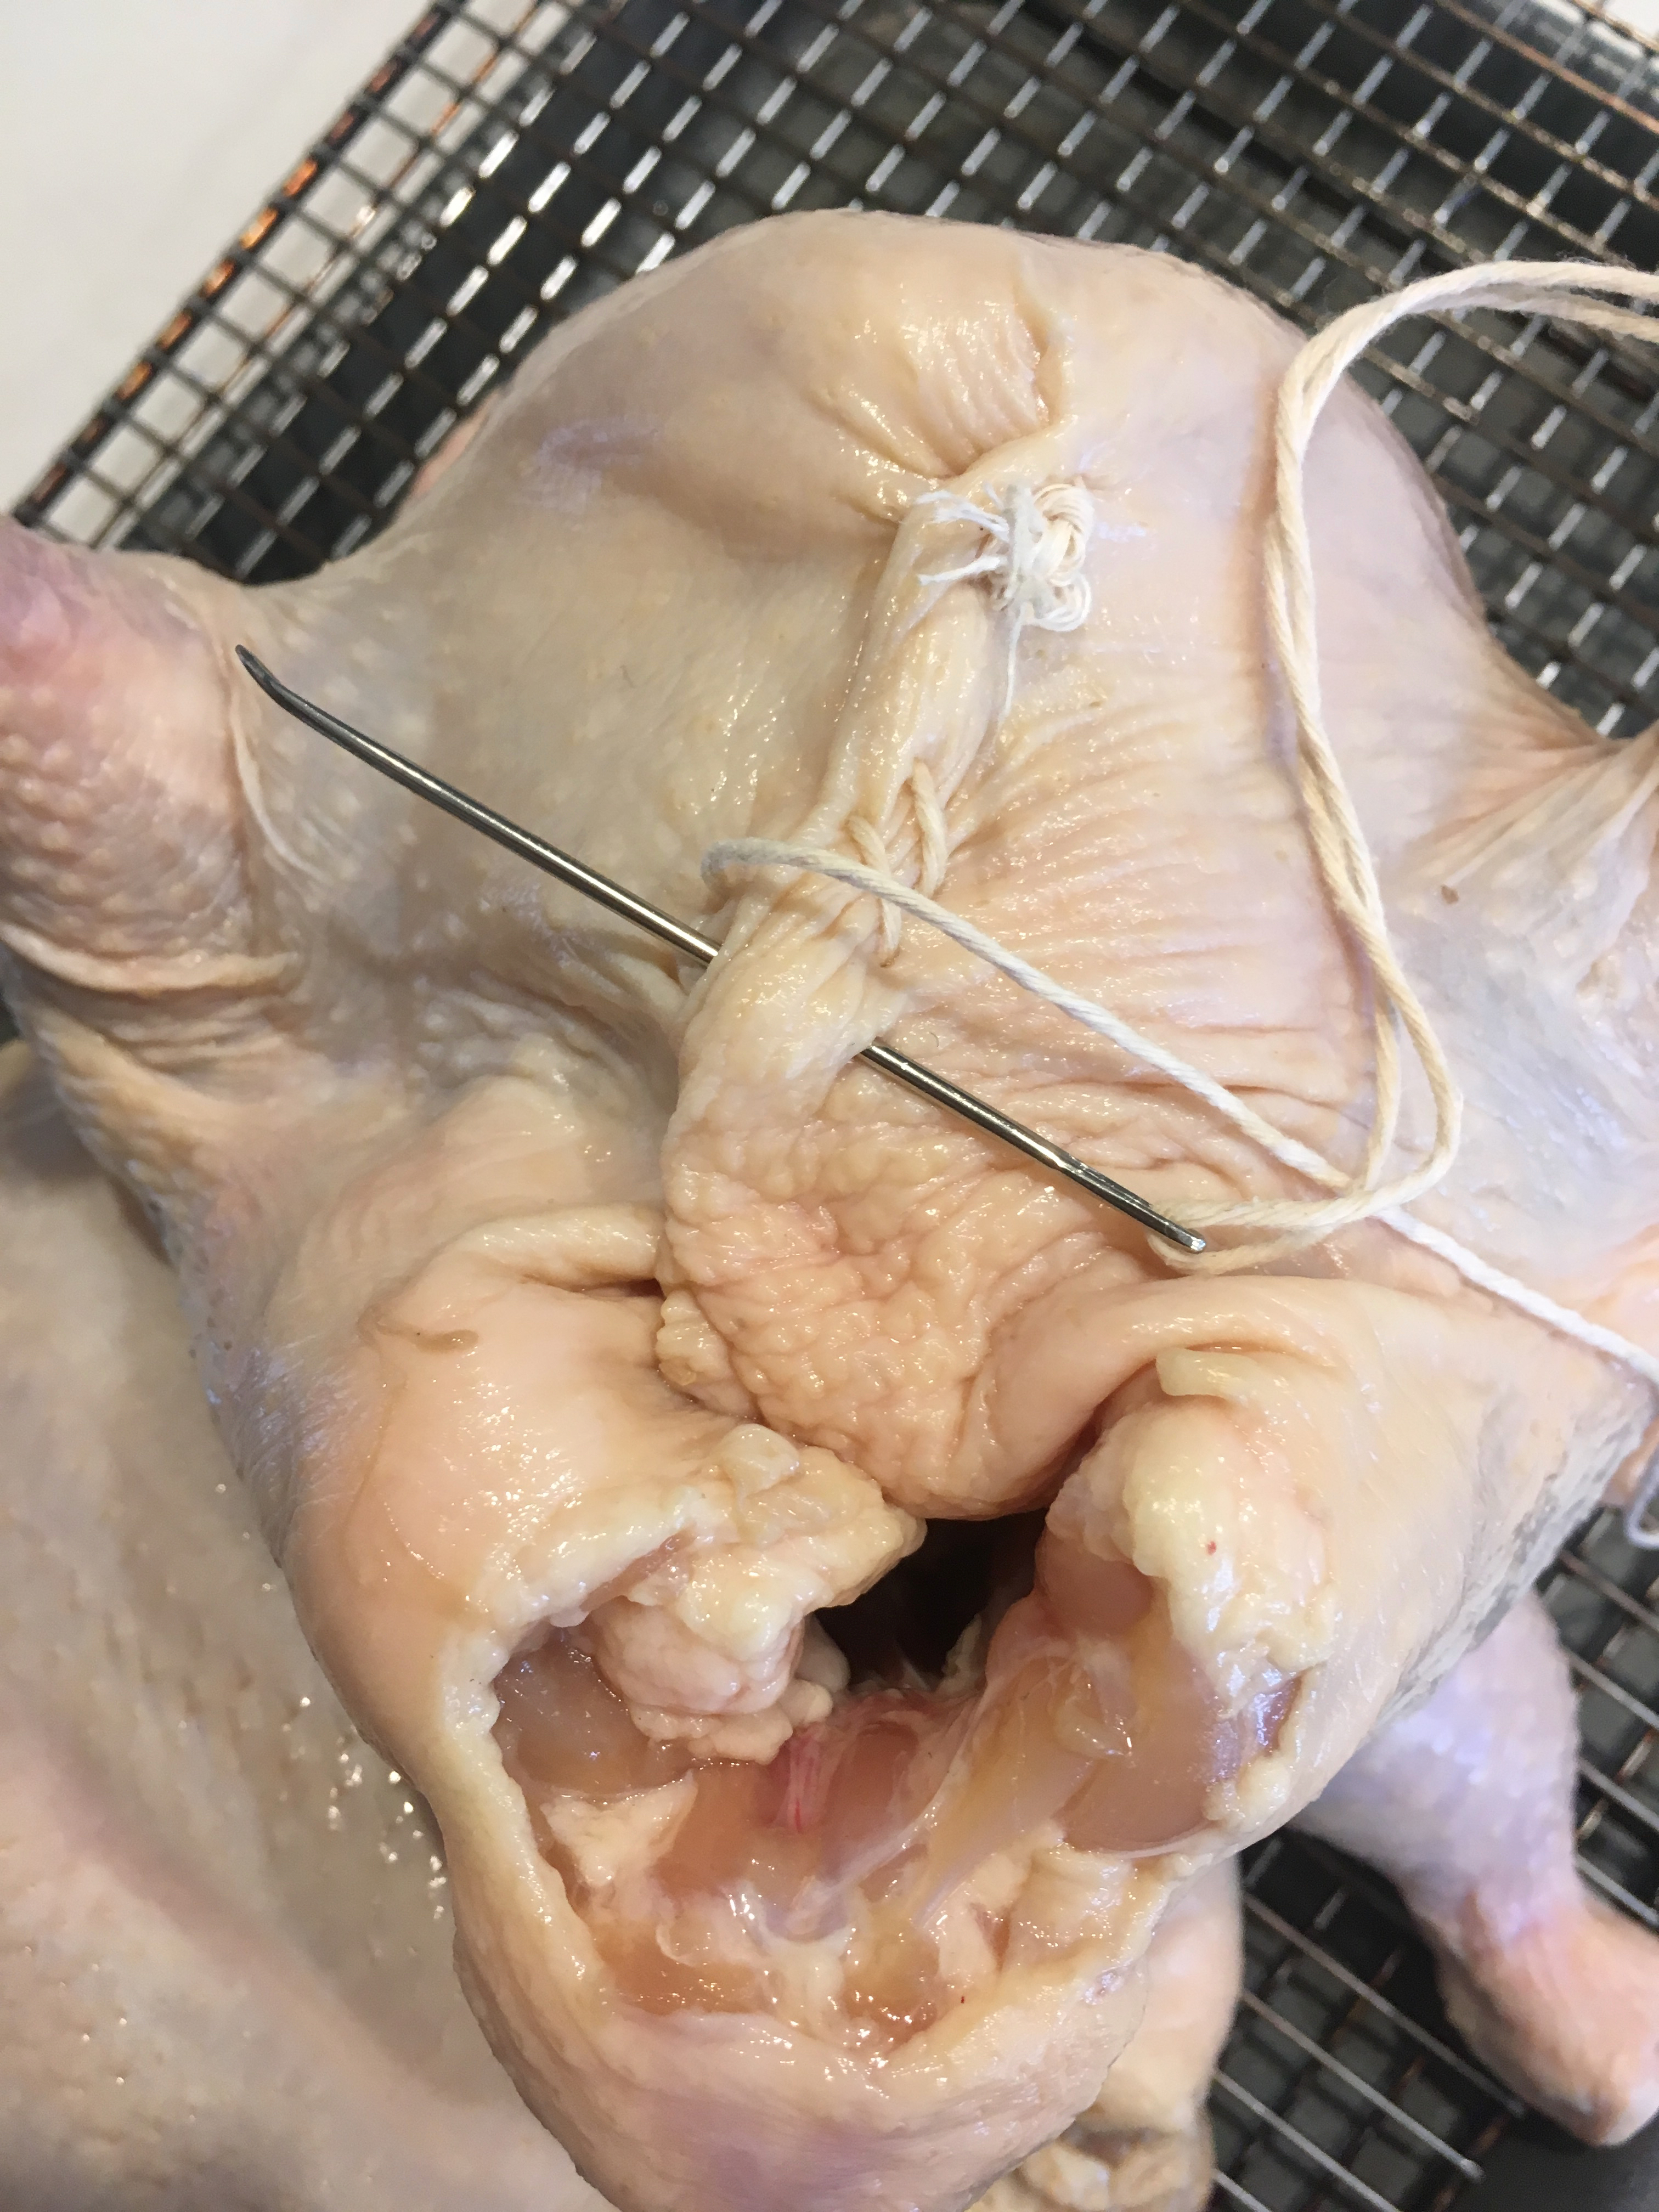
\includegraphics[width=0.25\textwidth]{\imageDir/\fileName/IMG_3214.jpg} &
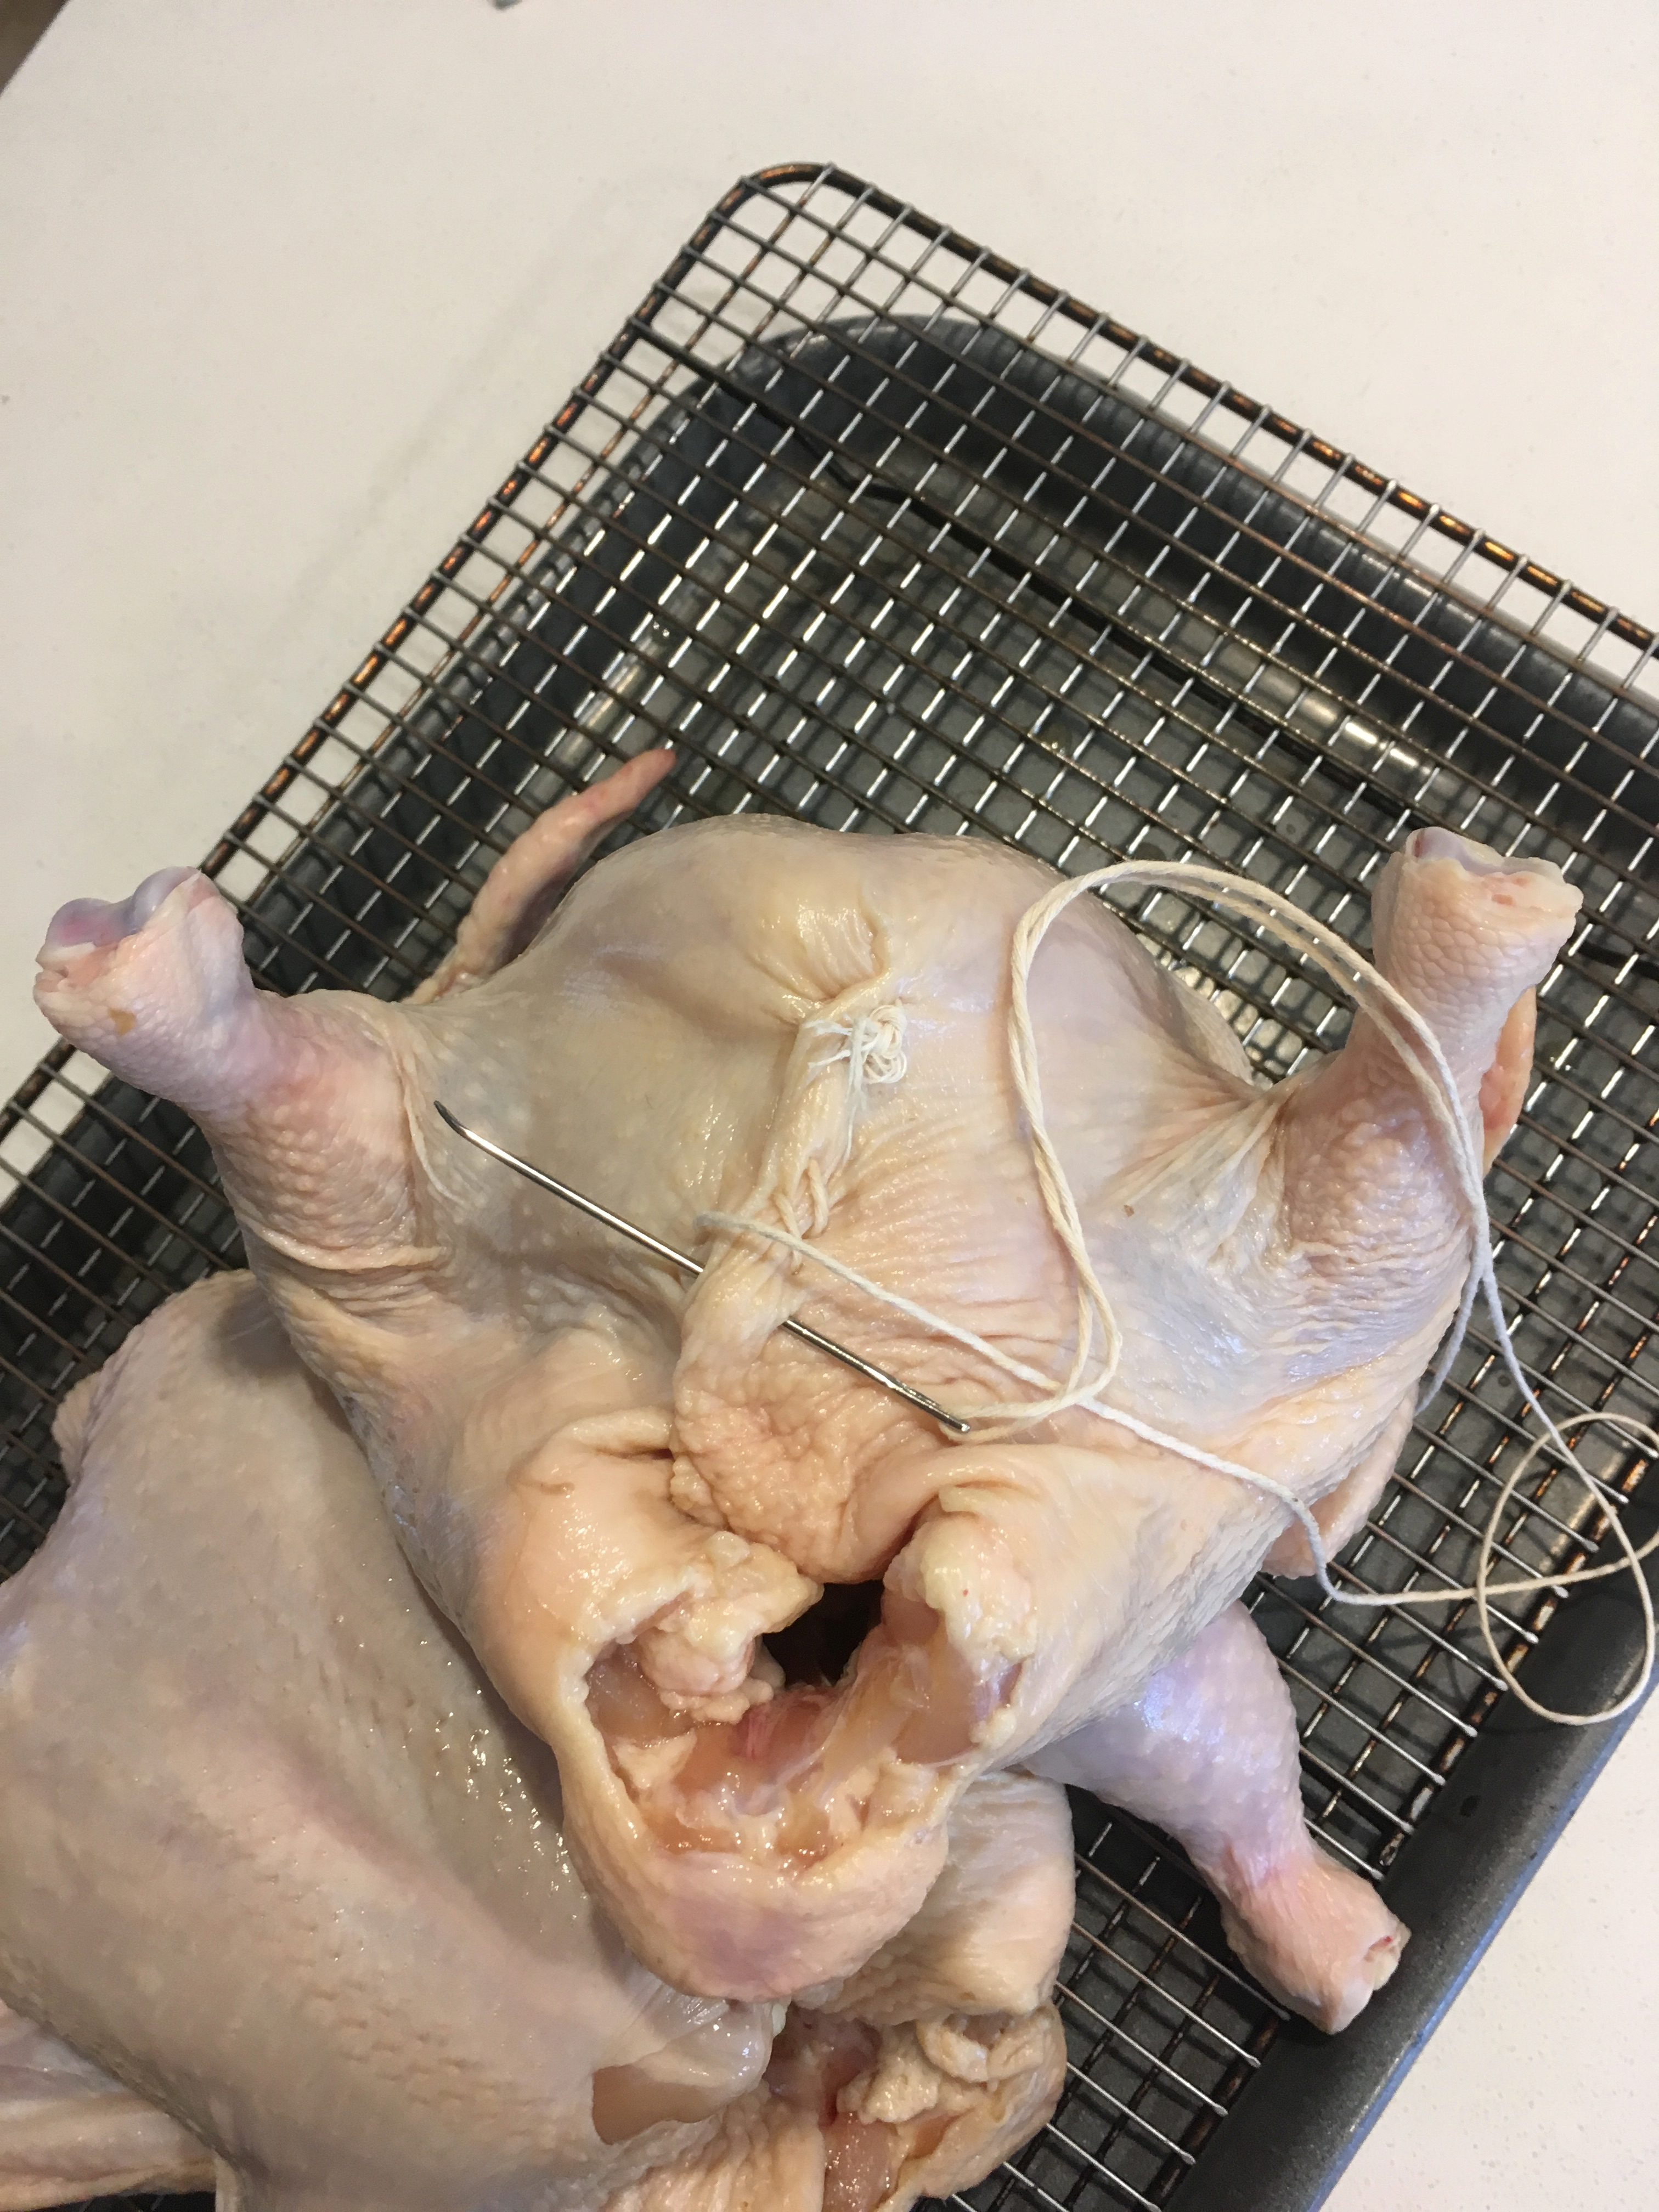
\includegraphics[width=0.25\textwidth]{\imageDir/\fileName/IMG_3216.jpg} \\
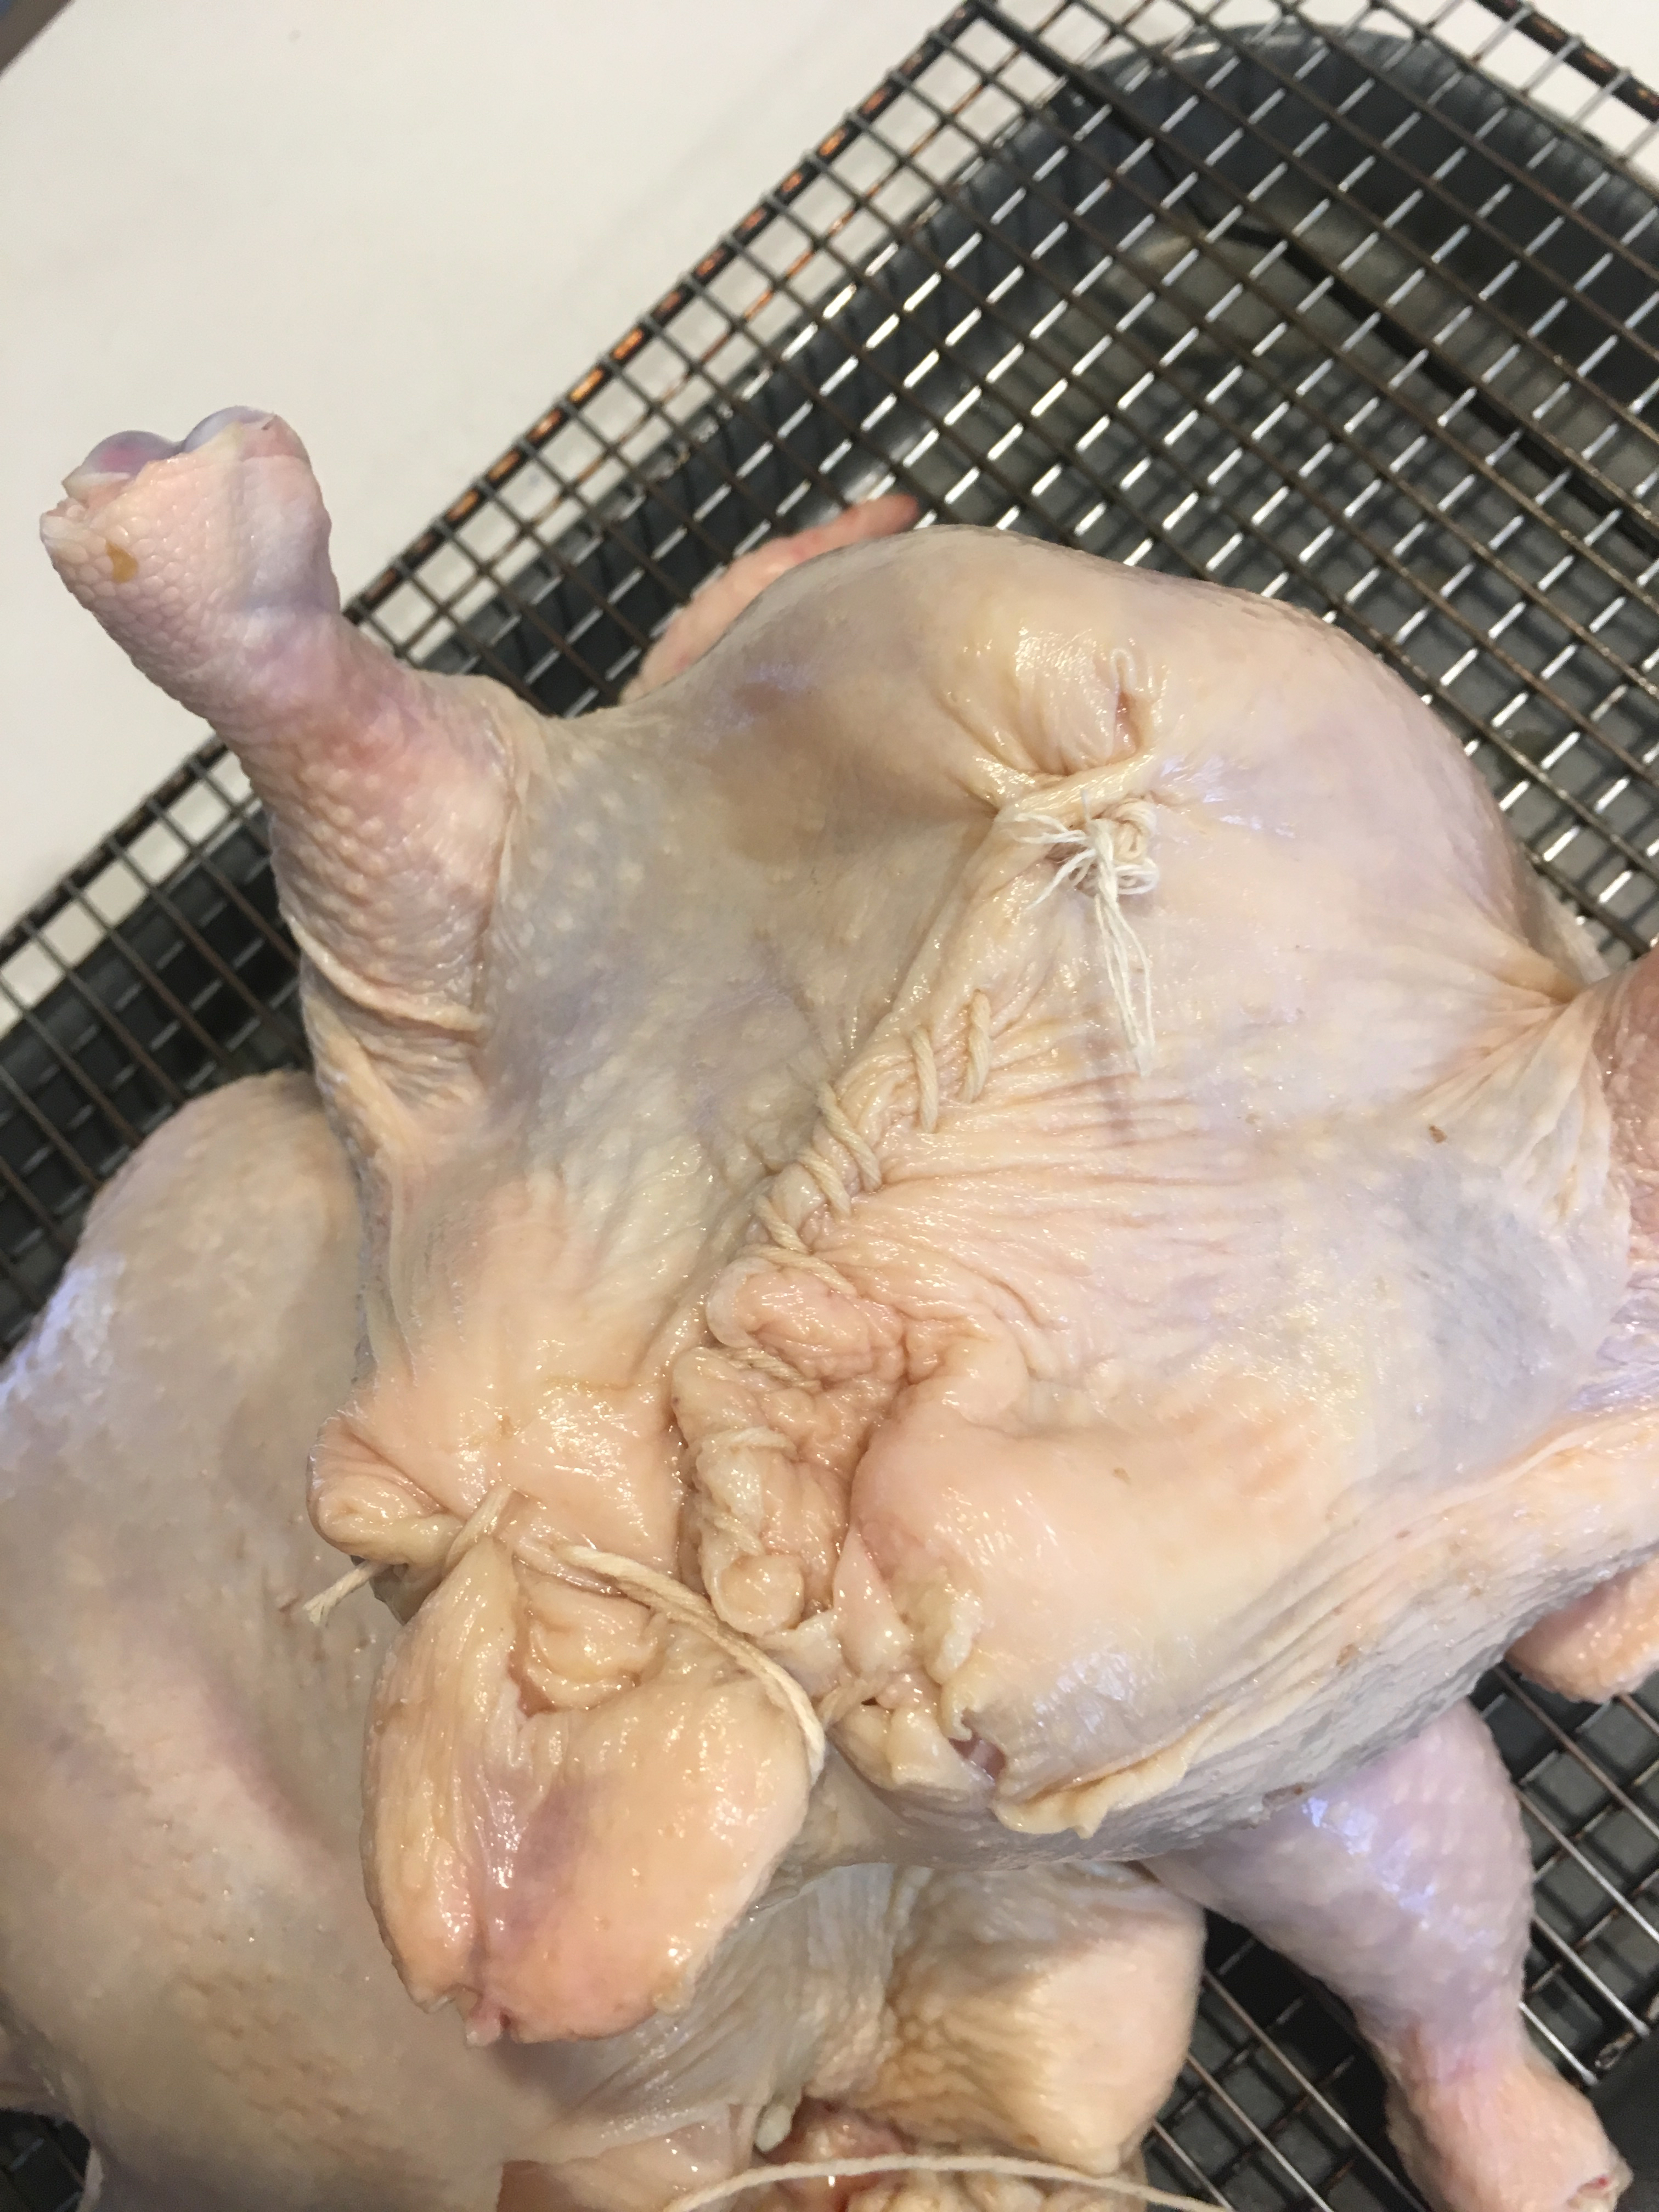
\includegraphics[width=0.25\textwidth]{\imageDir/\fileName/IMG_3217.jpg} &
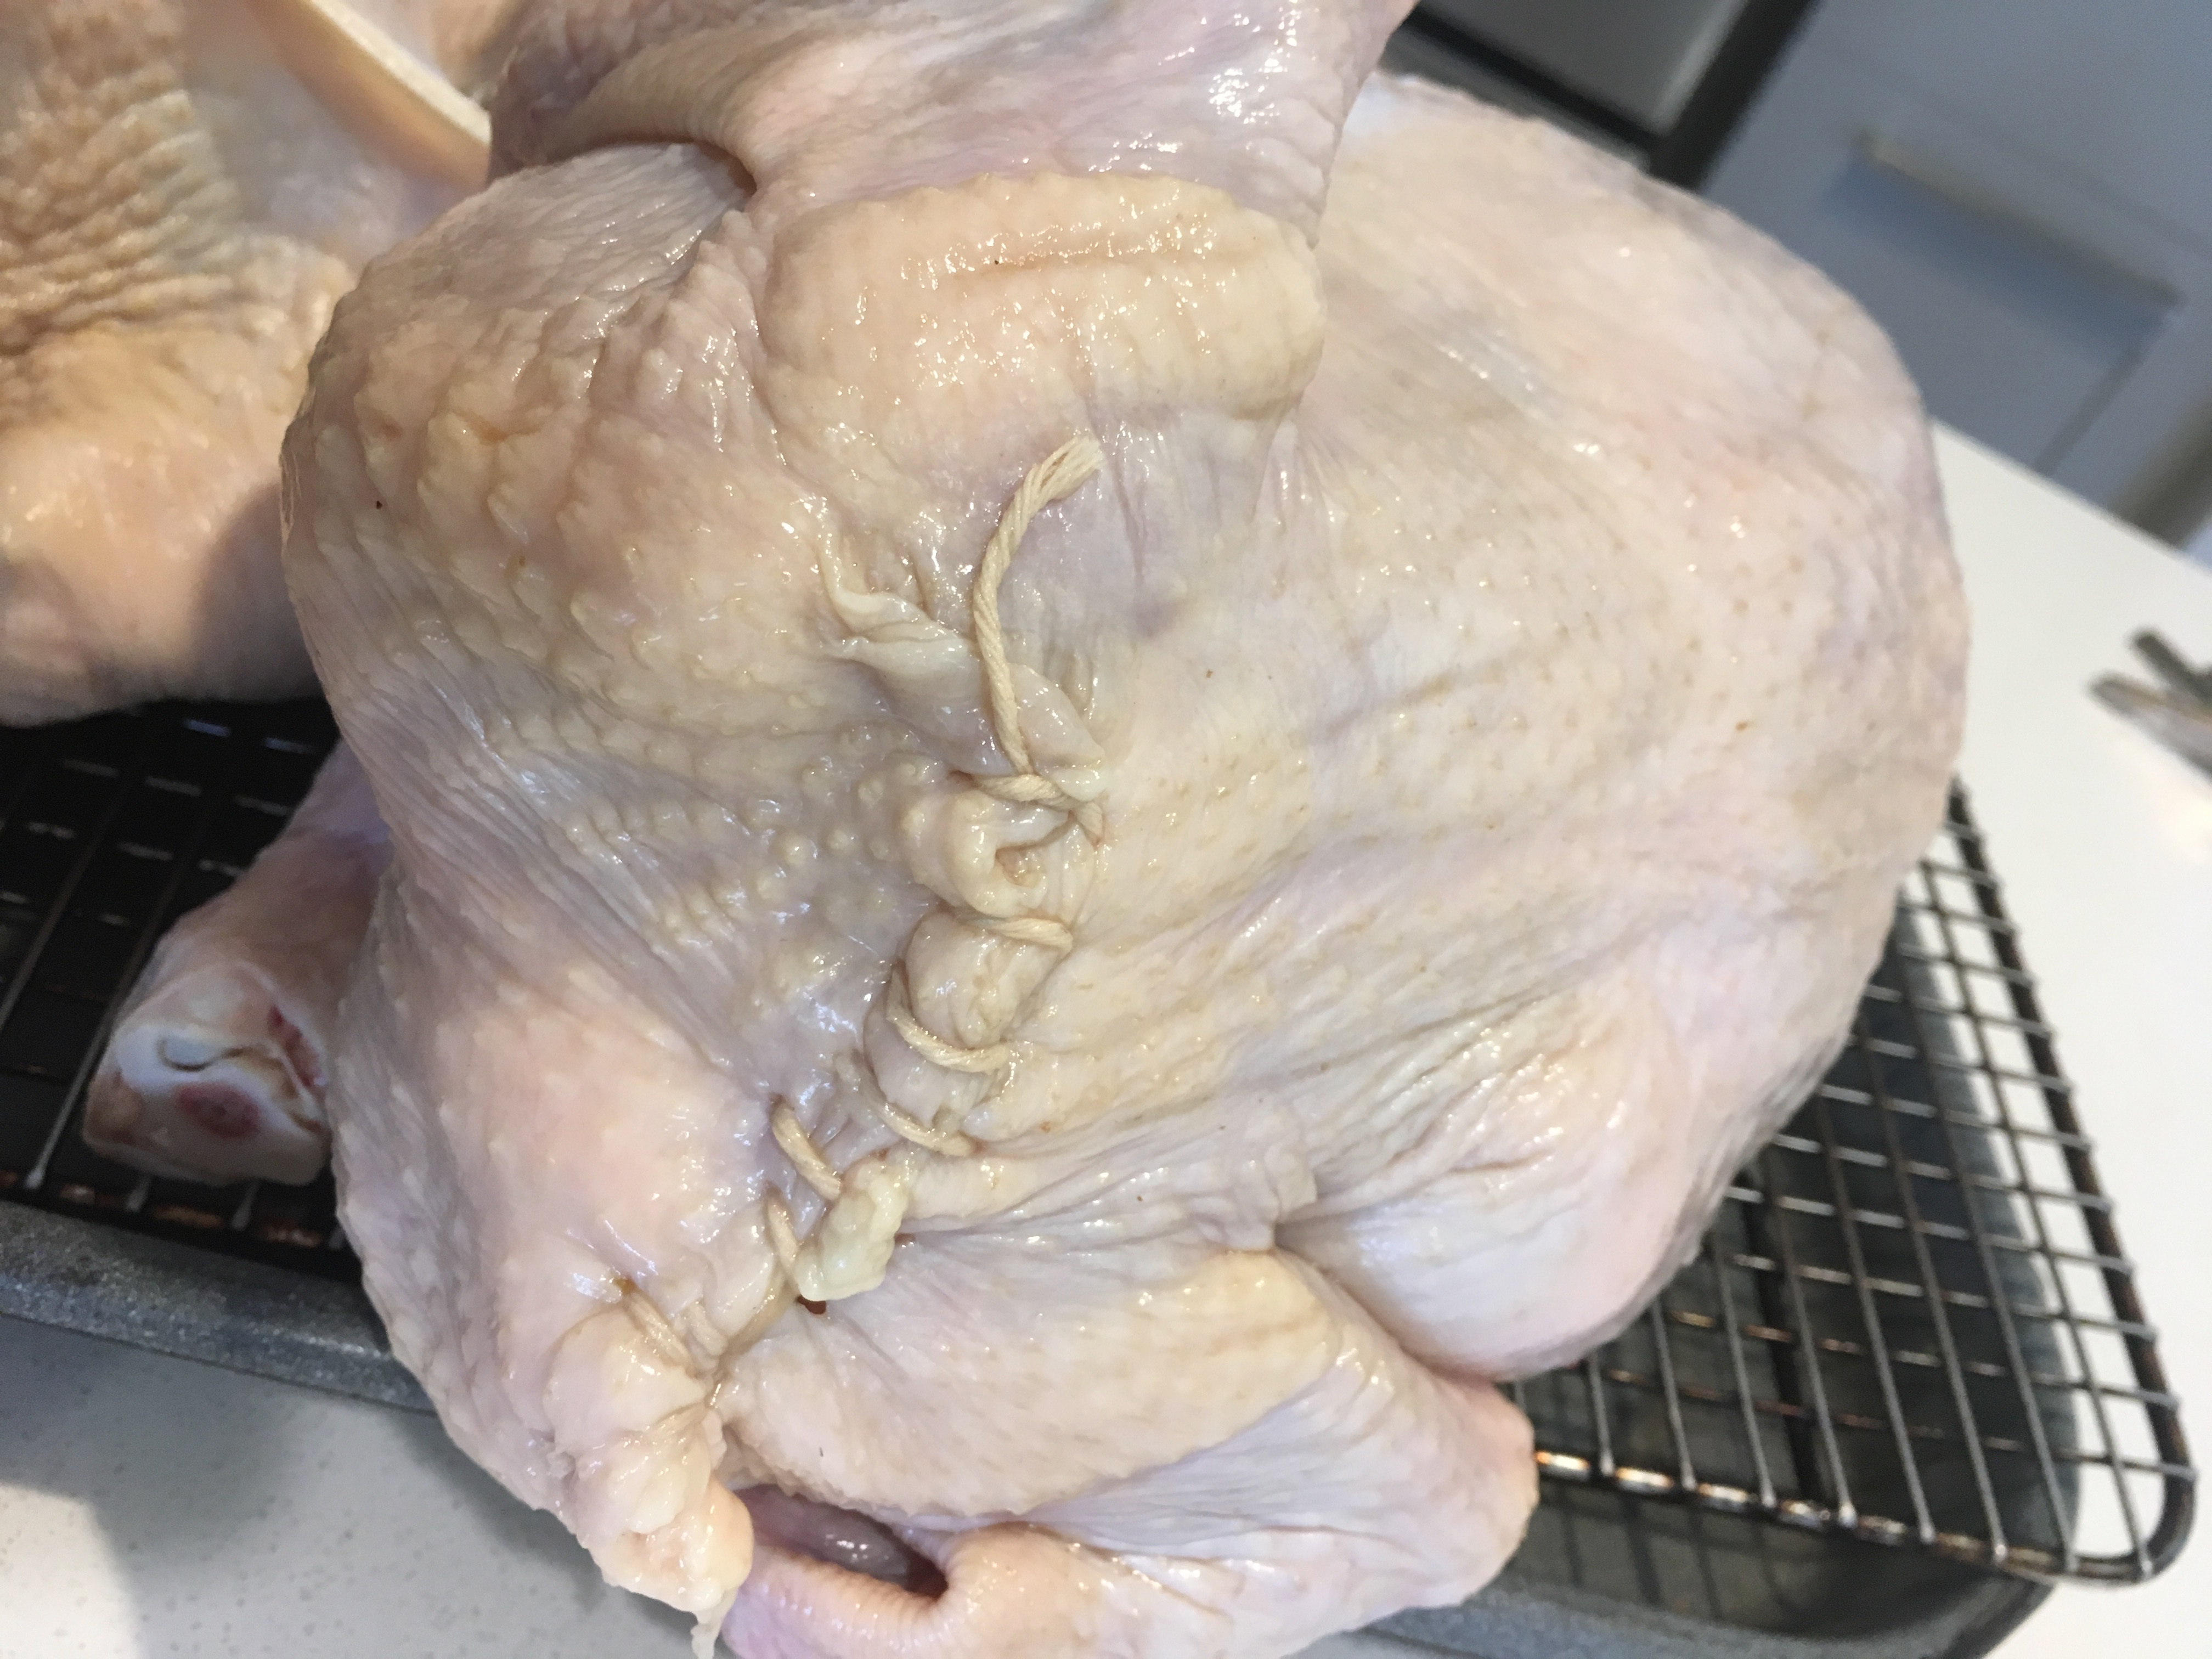
\includegraphics[width=0.25\textwidth]{\imageDir/\fileName/IMG_3218.jpg} &
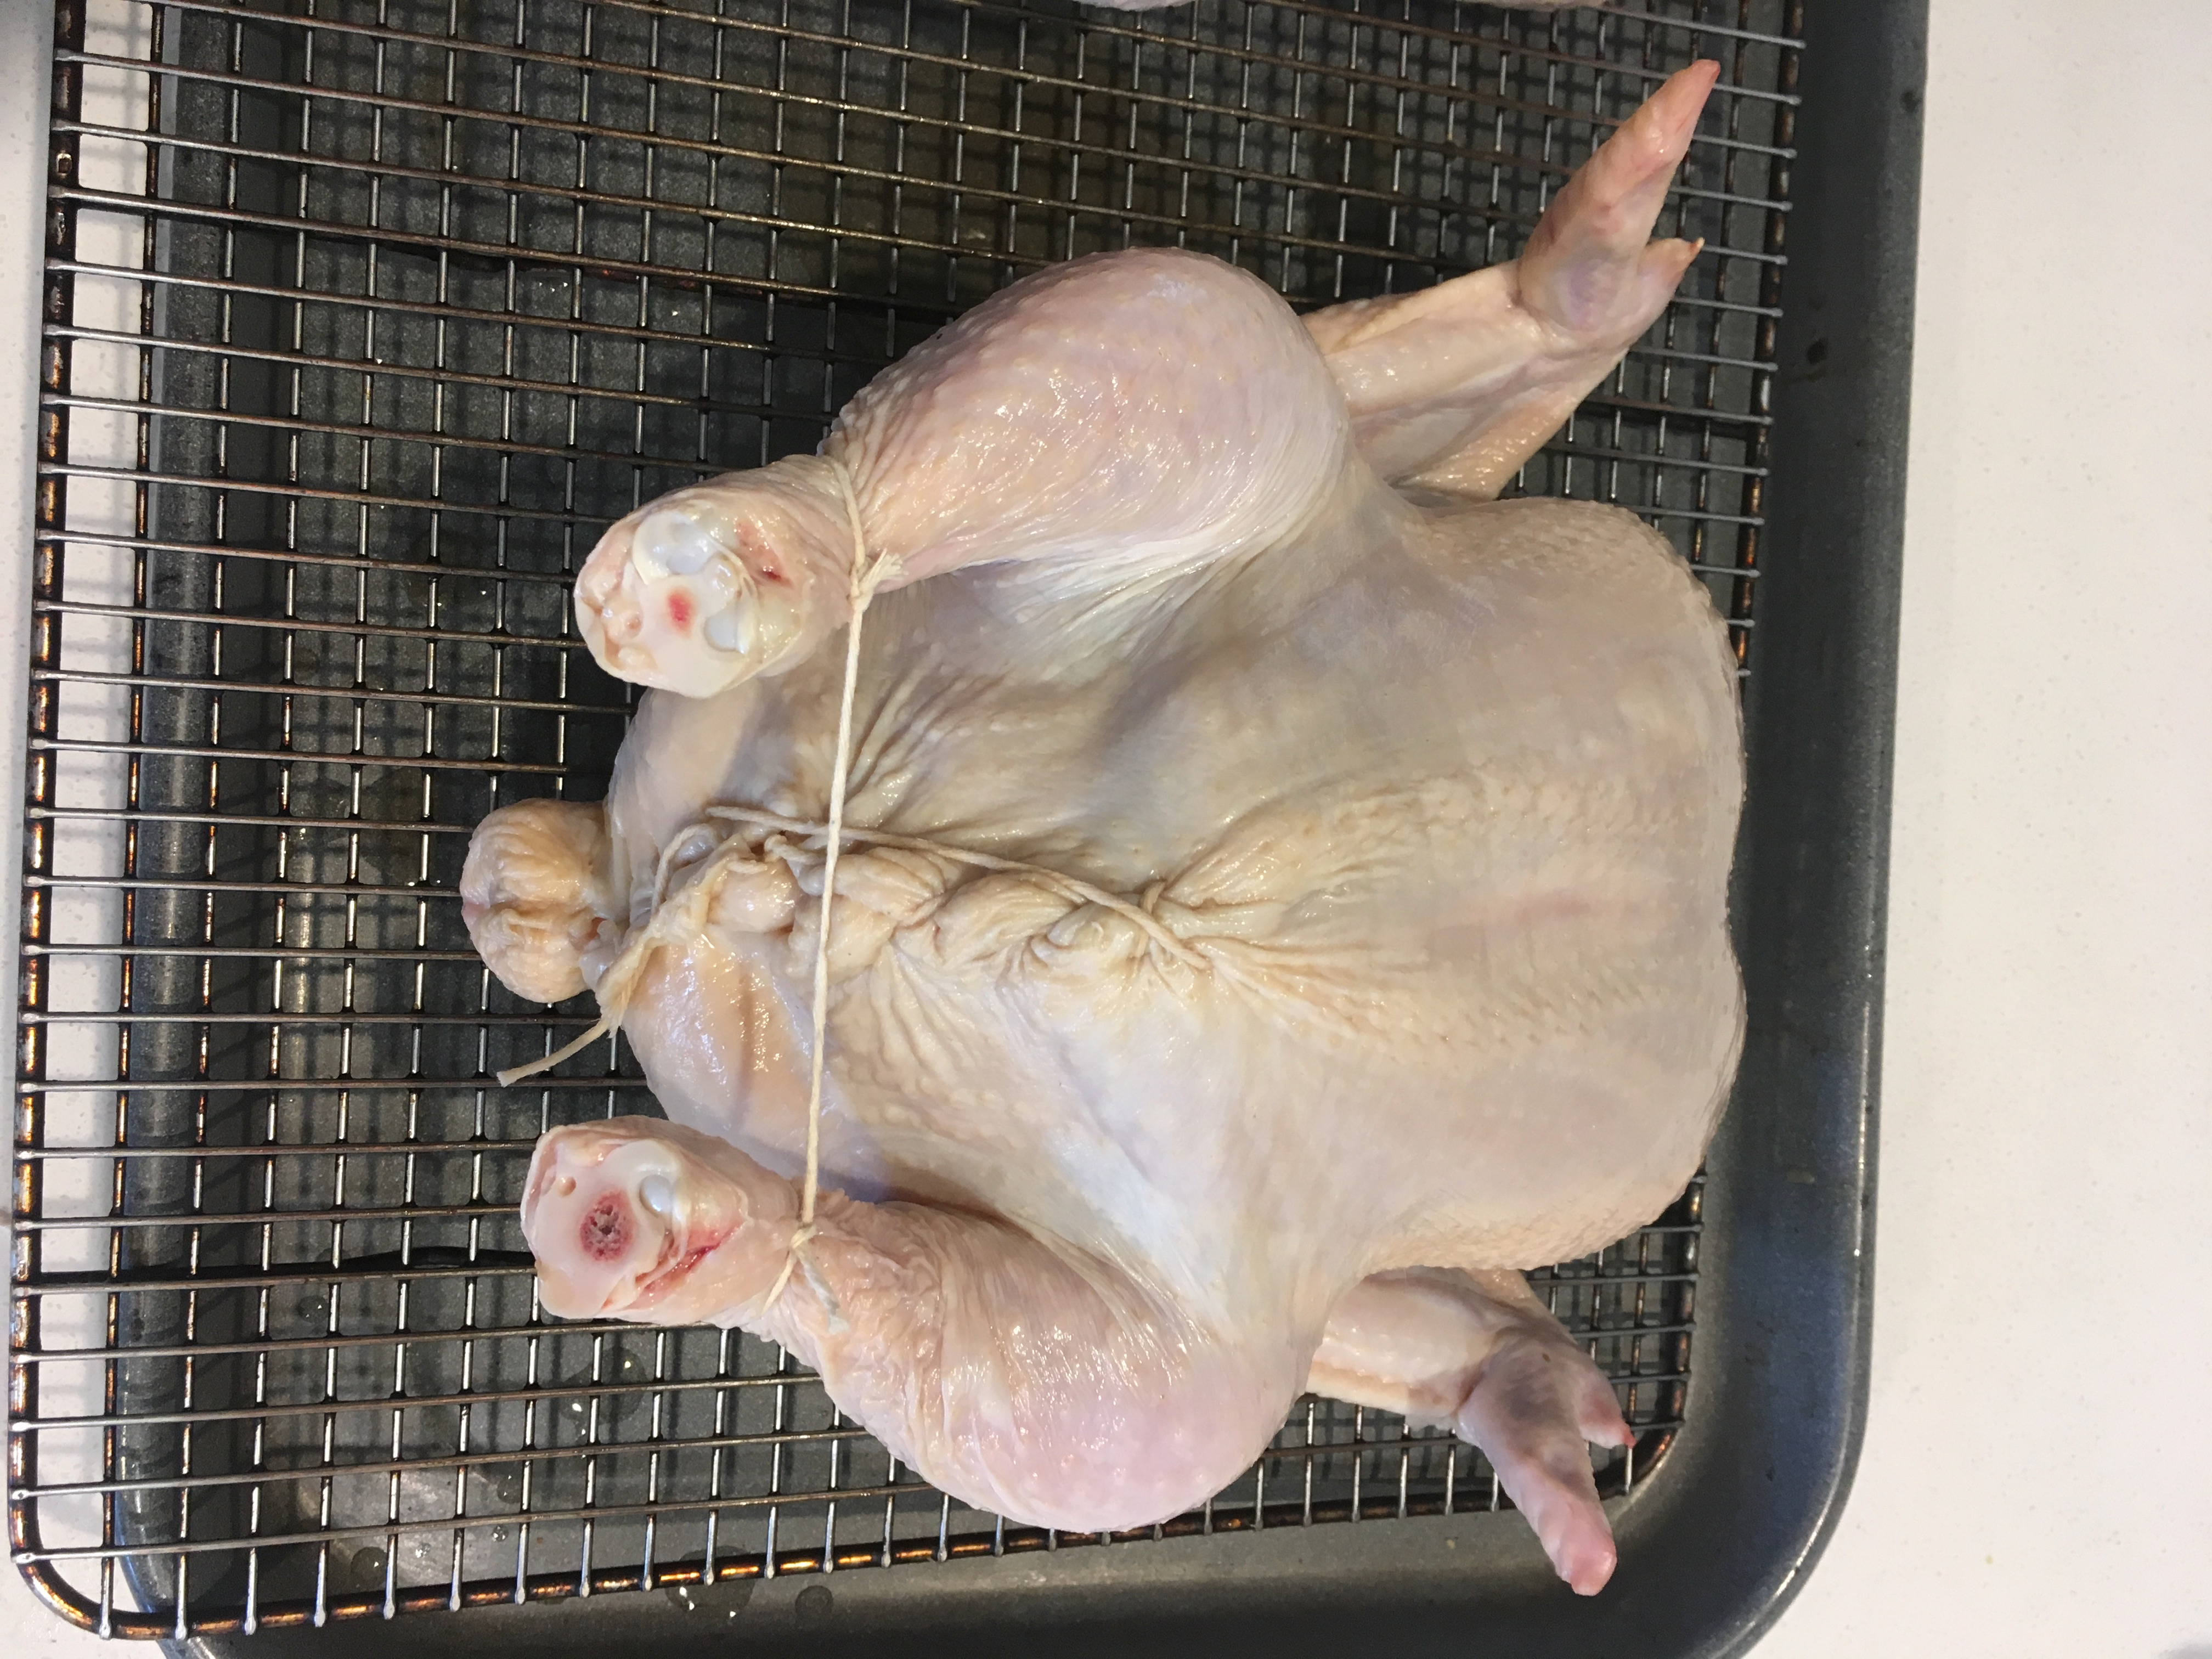
\includegraphics[width=0.25\textwidth]{\imageDir/\fileName/IMG_3219.jpg} \\
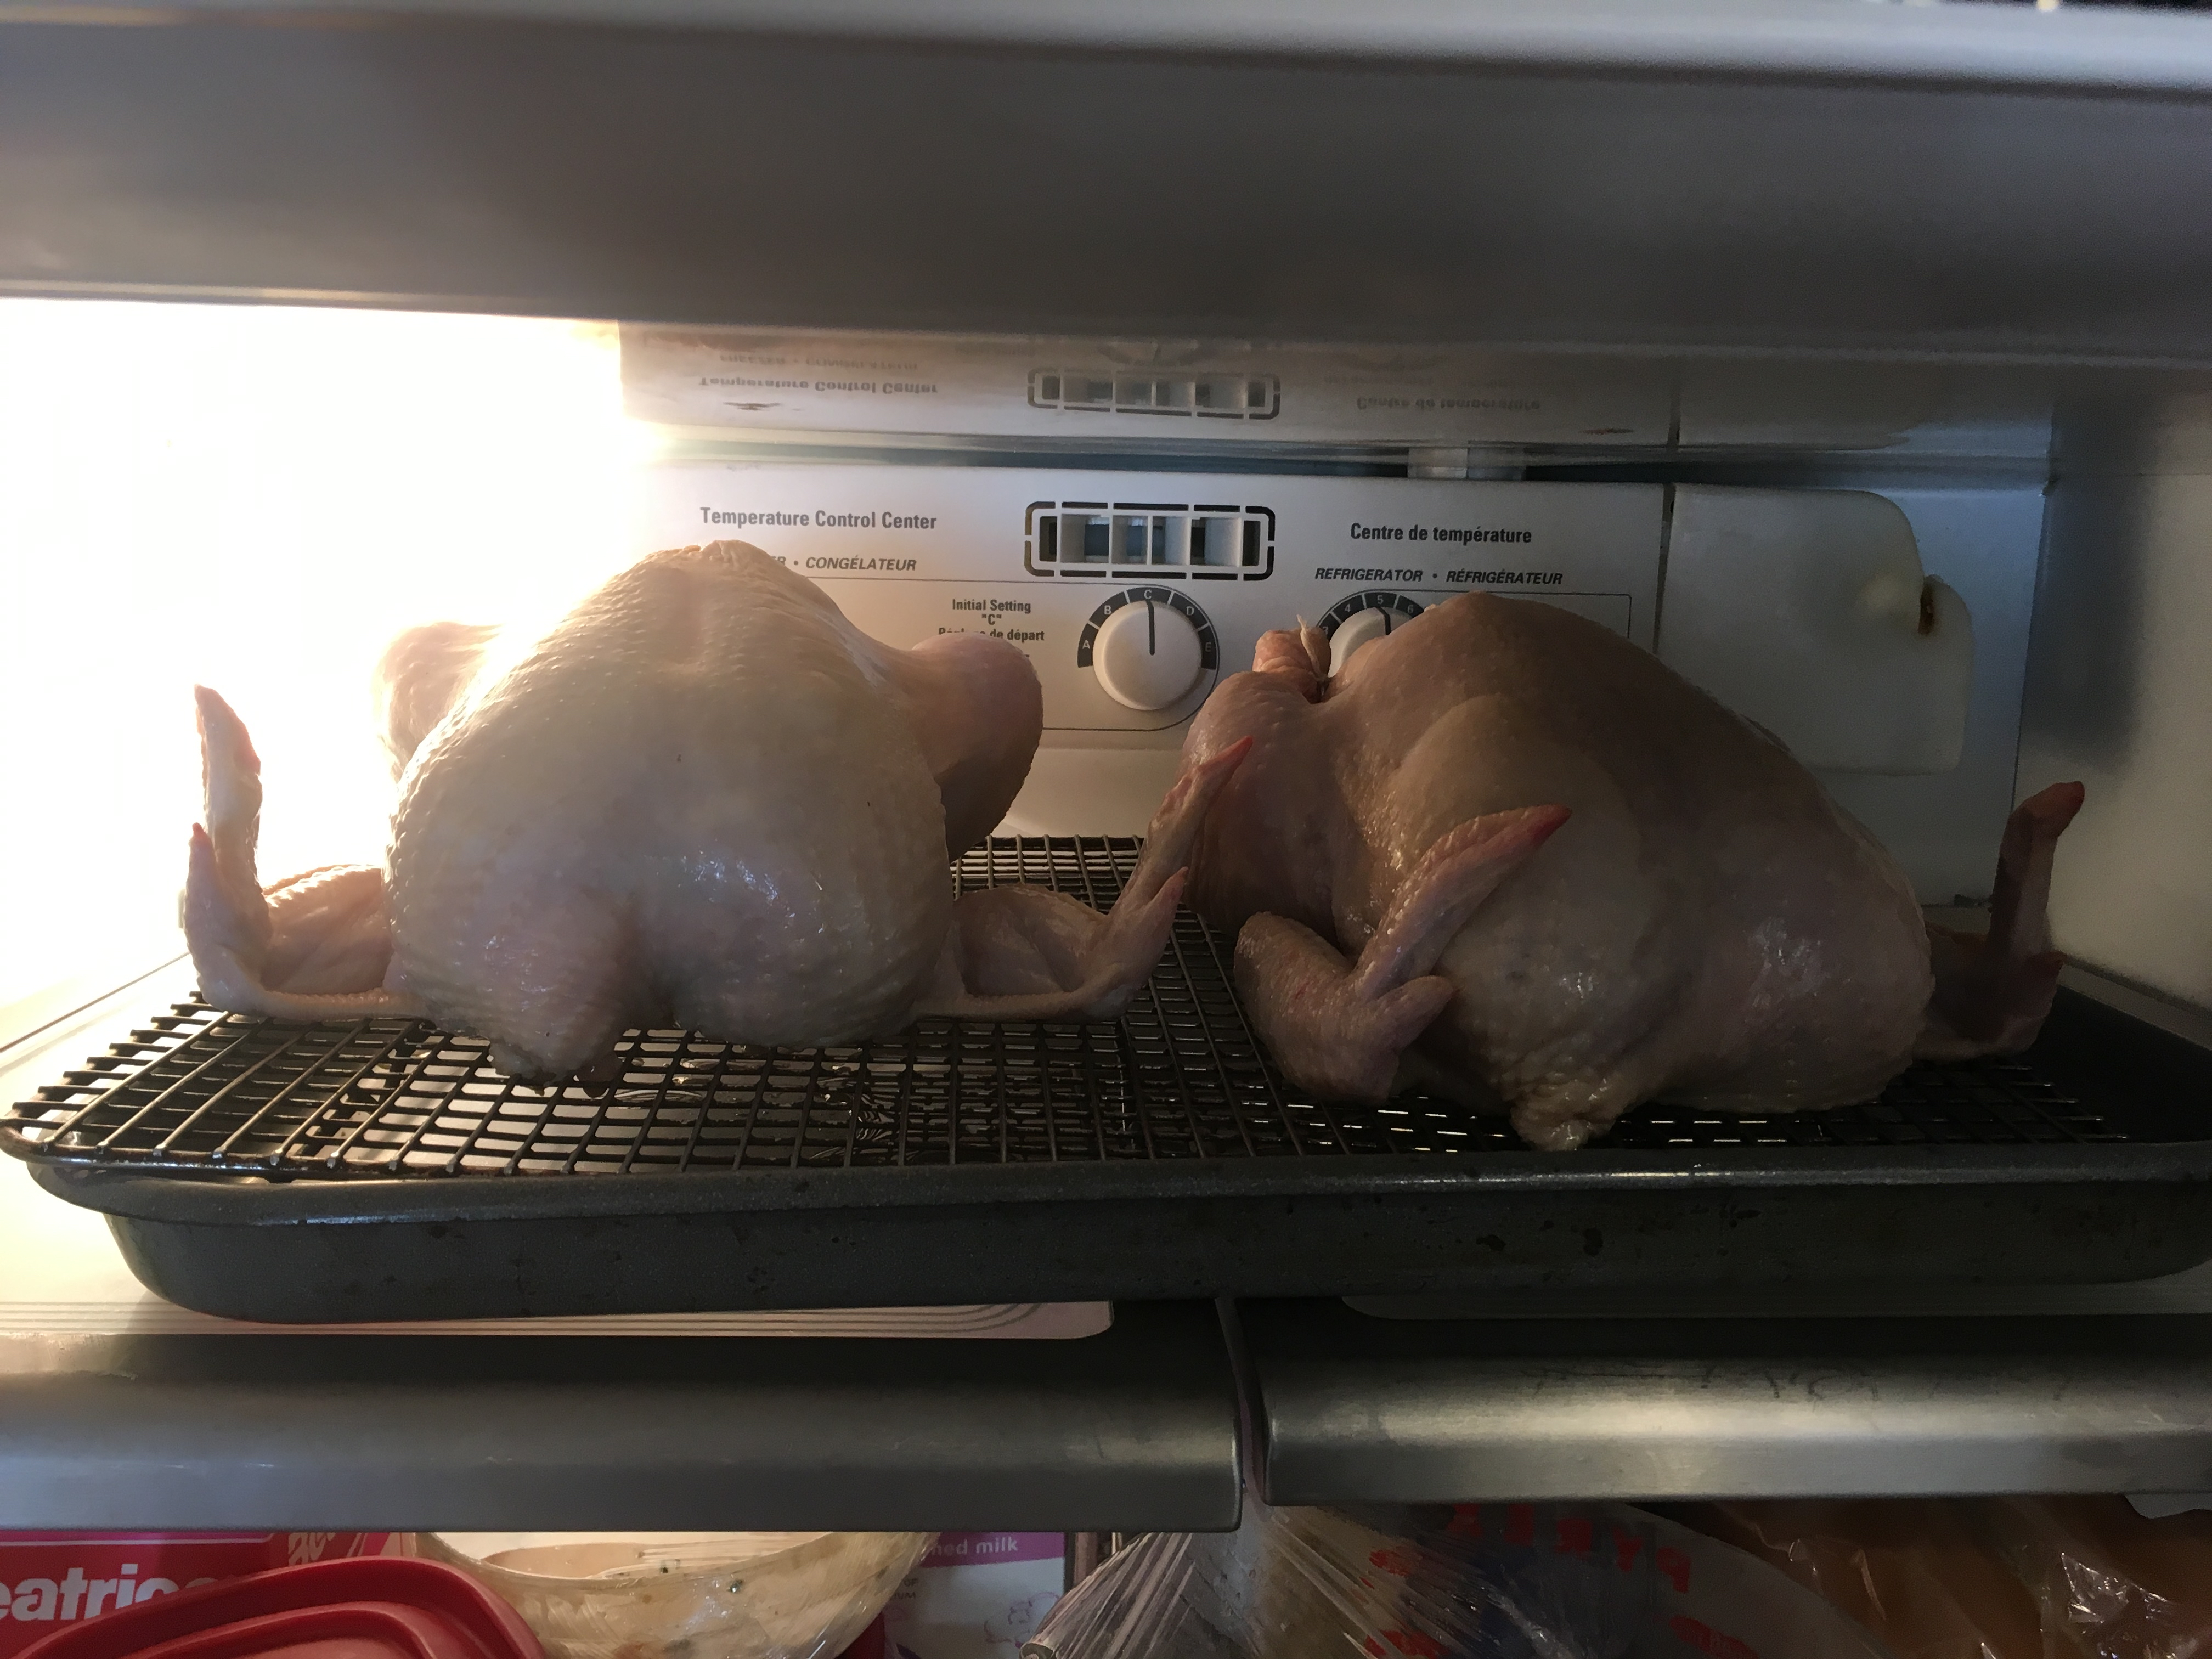
\includegraphics[width=0.25\textwidth]{\imageDir/\fileName/IMG_3220.jpg} &
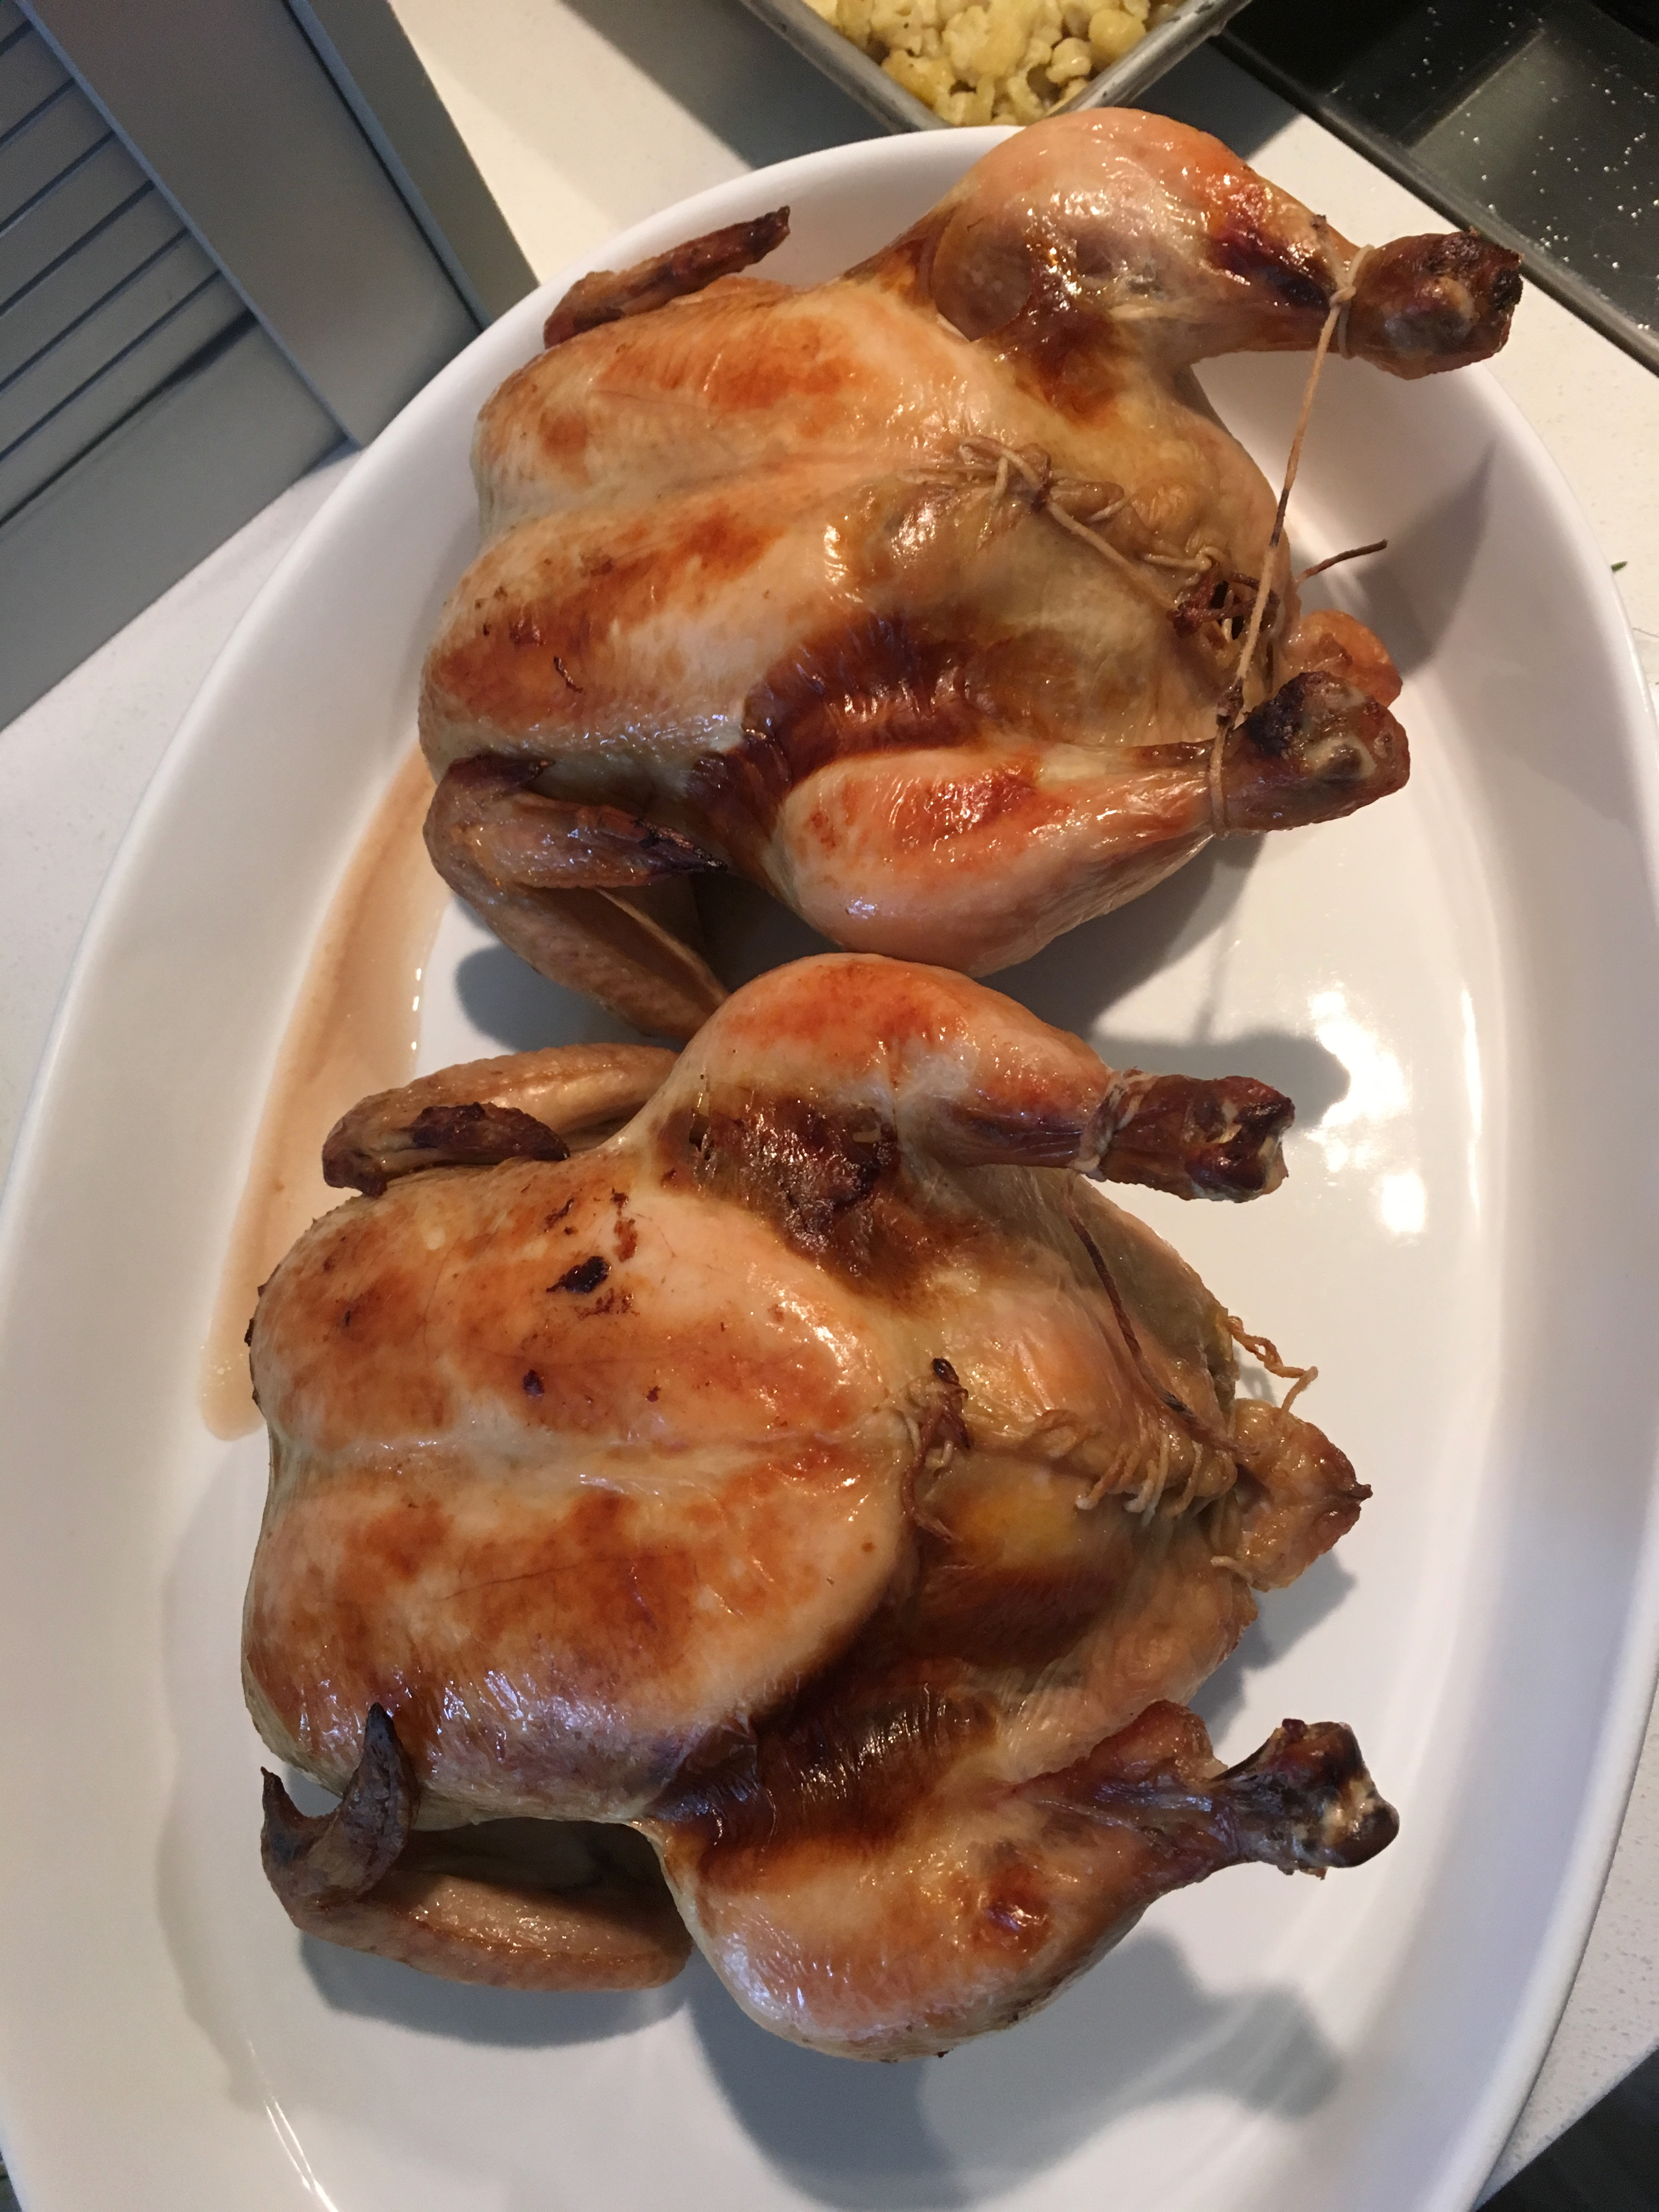
\includegraphics[width=0.25\textwidth]{\imageDir/\fileName/IMG_3228.jpg} \\
\end{tabular}
\end{table}

\end{document}
